%%%%%%%%%%%%%%%%%%%% file editor.tex %%%%%%%%%%%%%%%%%%%%%%%%%%%%%%%
%
% sample root file for a complete "contributed book"
%
% "contributed book"
%
% Copy it to a new file with a new name and
% use it as a template for your own input.
%
%%%%%%%%%%%%%%%%%%%%%%%% Springer-Verlag %%%%%%%%%%%%%%%%%%%%%%%%%%


\documentclass{svmult}

% choose options for [] as required from the list
% in the Reference Guide, Sect. 2.2

\usepackage{subfigure}
\usepackage{makeidx}         % allows index generation
\usepackage{graphicx}        % standard LaTeX graphics tool
                             % when including figure files
\usepackage{multicol}        % used for the two-column index
\usepackage[bottom]{footmisc}% places footnotes at page bottom

\usepackage[boxed]{algorithm2e} %% This is used in chapter 13 (LAAS Architecture)

% etc.
% see the list of further useful packages
% in the Reference Guide, Sects. 2.3, 3.1-3.3

\makeindex             % used for the subject index
                       % please use the style sprmidx.sty with
                       % your makeindex program


%%%%%%%%%%%%%%%%%%%%%%%%%%%%%%%%%%%%%%%%%%%%%%%%%%%%%%%%%%%%%%%%%%%%%
\begin{document}



\frontmatter%%%%%%%%%%%%%%%%%%%%%%%%%%%%%%%%%%%%%%%%%%%%%%%%%%%%%%

\thispagestyle{empty} \vspace*{3.5cm}
\begin{center}

% write your text here
{\huge Software Engineering}

\vspace*{0.5cm}

{\huge for Experimental Robotics}

\vspace*{3.5cm}

{\large Springer Tracts on Advanced Robotics}

\vspace*{1.5cm}

{\large Edited by Davide Brugali}


\end{center}

\mainmatter%%%%%%%%%%%%%%%%%%%%%%%%%%%%%%%%%%%%%%%%%%%%%%%%%%%%%%%
\part{Robotic Software Frameworks}
%%%%%%%%%%%%%%%%%%%%%%%%%% author.tex %%%%%%%%%%%%%%%%%%%%%%%%%
%
% sample root file for your contribution to a
%
% "contributed book" (global)
%
% Use this file as a template for your own input.
%
%%%%%%%%%%%%%%%%%%%%%%%% Springer-Verlag %%%%%%%%%%%%%%%%%%%%%%%%%%


%%% The following preamble of the contribution has been commented out
%%% to allow LaTeX to \include that document into the main book

% RECOMMENDED %%%%%%%%%%%%%%%%%%%%%%%%%%%%%%%%%%%%%%%%%%%%%%%%%%%
%\documentclass{svmult}

%% choose options for [] as required from the list
%% in the Reference Guide, Sect. 2.2

%\usepackage{makeidx}         % allows index generation
%\usepackage{graphicx}        % standard LaTeX graphics tool
                              % when including figure files
%\usepackage{multicol}        % used for the two-column index
%\usepackage[bottom]{footmisc}% places footnotes at page bottom
% etc.
% see the list of further useful packages
% in the Reference Guide, Sects. 2.3, 3.1-3.3

%\makeindex             % used for the subject index
                       % please use the style sprmidx.sty with
                       % your makeindex program


%%%%%%%%%%%%%%%%%%%%%%%%%%%%%%%%%%%%%%%%%%%%%%%%%%%%%%%%%%%%%%%%%%%%%

%\begin{document}

\title*{Research Directions in Robotic Software Frameworks}
% Use \titlerunning{Short Title} for an abbreviated version of
% your contribution title if the original one is too long
\author{Davide Brugali\inst{1}\and Antonio Cisternino\inst{2}
\and Diego Colombo\inst{2} \and Carle C�t�\inst{3}\and Jannik
Fritsch\inst{4}\and Brian Gerkey\inst{5} \and Gerhard
Kraetzschmar\inst{6} \and Fran�ois Michaud\inst{3} \and Richard
Vaughan\inst{7}\and Hans Utz\inst{8}}
\authorrunning{Brugali et al.}
\institute{Universit\'a degli Studi di Bergamo, Italy \texttt{brugali@unibg.it} 
\and AAA \texttt{aaa@bbb.bb} 
\and AAA \texttt{aaa@bbb.bb}
\and AAA \texttt{aaa@bbb.bb}
\and SRI International, USA \texttt{gerkey@ai.sri.com} 
\and AAA \texttt{aaa@bbb.bb}
\and Simon Fraser University, Canada \texttt{vaughan@sfu.ca}
\and AAA \texttt{aaa@bbb.bb}}


%
% Use the package "url.sty" to avoid
% problems with special characters
% used in your e-mail or web address
%
\maketitle

\section{Introduction}
\label{sec:ch31-Intro}

In the software community, a framework indicates an integrated set
of domain-specific software components
\cite{31_CoplienSchmidt1995} which can be reused to create
applications. A framework is more than a library of software
components: It defines the common architecture underlying the
particular applications built on the framework. Frameworks are a
powerful development approach as they consist of both reusable
code (the component library) and reusable design (the
architecture).

Frameworks have acquired popularity in object-oriented (OO). Here,
the interpretation of "framework" ranges from structures of
classes of cooperating objects, which through extension provide
reusable basic designs for a family of similar applications
\cite{31_JohnsonFoote1988}, to the more restrictive view
\cite{31_Schmid1995} of complete, high level modules, which
through customization directly result in specific applications for
a certain domain. Customization is done through parameterization
or by writing functional specifications.

Frequently, the two views of framework, referred to as white box
and black box approaches to reuse, may be simultaneously present
in one framework. In fact, features which are likely to be common
to most applications can be offered and therefore reused as black
boxes. Black-box frameworks support extensibility by defining
interfaces for components that can be plugged into the framework
via composition. Existing functionalities are reused by defining
components that conform to a particular interface and integrating
these components into the framework. On the other hand, the class
library accompanying the framework usually provides base classes
(seen as white boxes) that can be specialized, by adding
subclasses as needed, and easily integrated with the rest of the
framework. White-box frameworks rely heavily on OO language
features like inheritance and dynamic binding in order to achieve
extensibility. Existing functionality is reused and extended by
(1) inheriting from framework base classes and (2) overriding
predefined hook methods using design patterns like the Template
Method \cite{31_Gamma1995}.

Framework based development has two main processes: development of
the framework and development of an application adapting the
framework. Every application framework evolves over time; this is
called the framework life span \cite{31_Brugali1997}. Within this
life span, the basic architectural elements which are independent
from any specific application are implemented first. When new
applications are built using the framework, new components are
developed which eventually are generalized and integrated as new
black box elements. This means that in its early stages a software
framework is mainly conceived as a white box framework. However,
through its adoption in an increasing number of applications, the
framework matures: More concrete components, which provide black
box solutions for common difficult problems, as well as high level
objects, which represent the major abstractions found in the
problem domain, become available within the framework.

Since developing the framework requires a lot of effort, it is
justified only if several applications will be built based on the
framework. On the other hand, when the framework is available,
developing an application from it offers considerable saving in
time and effort compared to the development from scratch. The
application is built by slightly modifying the framework, but by
accepting the framework's high level design in general. In other
words, most of the framework is reused, and reuse happens both at
the high level design and at the code level. Building a framework
is more demanding than building an application. The designer has
to have a deep understanding of the domain the application is
embedded into, and has to anticipate the needs of future
application developers. As a matter of fact, successful frameworks
are often derived from reengineering legacy applications by
abstracting from them the knowledge of principal software
designers.

Most framework-based software development is organized along the
value-added principle \cite{31_Mili2002}. This divides any
software system into a set of horizontal layers, each one built on
top of another. This approach promotes separation of concerns and
enforces modularity. Typically, a software framework is subdivided
into a system infrastructure layer, a functional (also called
horizontal or business domain) layer, and an application (also
called vertical) layer.

The \emph{system infrastructure layer} (usually called
\emph{middleware}) consists of a collection of software components
that offer basic services like communication between distributed
applications, uniform access to heterogeneous resources,
independence from processing platforms and distributed location,
distributed component naming, service brokering and treading, and
remote execution. Examples of distributed middleware systems are
Microsoft .NET, the implementations of OMG CORBA, and the Sun
Enterprise Java Beans.

The customization of the system infrastructure layer is usually
black-box. It consists in the aggregation of the frameworks'
elemental components (such as mechanisms for logical
communication, concurrency, and device abstraction) in which the
whole application has to be written.

The \emph{functional} (also called \emph{business domain})
\emph{layer} is the model of a robotic application and consists of
software components, which directly map to real entities like a
vision system or to common robot functionalities such as sensor
processing, mapping, localization, path planning, and task
planning, or even to typical robot capabilities such as reactive
behaviors.

Typically, they are implemented on top of the system
infrastructure layer. For example, reactive behaviors delegate
device abstractions for motion actuation, sensor processing, path
planning, and task planning rely on the framework concurrency
model in order to execute on different time scale, multi-robot
mapping and localization build on data exchanged through a common
distributed environment.

The customization of the functional layer is usually white-box.
The basic components are intermediary classes, which by their very
nature are fairly application independent, although they have been
conceived bearing in mind a specific application domain (e.g.
robot mobility or visual servoing). They are written using the
elemental components of the framework, and they have to be
specialized for each concrete application.

The \emph{application layer} connects the functional components
according to the information and control flows of any robot task.
Examples of robot tasks are soccer playing, vacuum cleaning,
museum tour guiding, mars surface exploration.

The customization of the application layer is usually grey-box. It
consists of the interconnection of pluggable application-specific
components through the middleware system. These components are the
result of the adoption of the framework for the development of
more and more applications and in some cases they are open source
components-off-the-shelf (COTS). COTS products are designed to
support a standard virtual interface, which consists of a set of
rules for accessing the component's functionality in a homogeneous
way, regardless of the execution platform, the programming
language, and other specifics.

Software frameworks offer a unified view to model and develop
robotic software systems at every level of the vertical
decomposition from the system infrastructure to the final
application through the functional model.

The papers in the third Part of this book describe different
approaches that address to some extent most or all of the aspects
of robot framework development (such as black box or white box
reuse. Individually, they propose innovative contributions on how
to apply framework development concepts in the robotics domain.
These approaches are illustrated in the next section. Thereafter,
the final section draws some conclusions.


\section{Opportunities to exploit Framework-based development in Robotics}
\label{sec:ch31-Opportunities}

Robot software developers have often experienced a sense of
frustration when developing an application that is (nearly) the
same as several other releases for different projects, but they
have not been able to capture and exploit the commonalties. These
problems frequently and typically occur in four circumstances.

\begin{enumerate}
\item When the application migrates to a different robot platform.
Despite the differences in the mechanical structure, many
commonalties can be identified in the control architecture, such
as how to acquire sensory data or transmit commands to the
actuators.

\item When the application scales up from a single robot to a
multi-robot system or when it is restructured from centralized to
decentralized and distributed control paradigm. Despite the
differences in the communication mechanisms (shared memory or
networked environment) the interactions among the control modules
of the robot control architecture remain unchanged or show many
commonalties.

\item When the same robotic system is used in different environments or
for different tasks. Despite the differences in the control logic,
most of the robot capabilities and functionalities are common in
every application.

\item When the robotic system is build from the composition of
heterogeneous or legacy subsystems. Despite the differences in the
programming languages, concurrency models, or data interchange
formats, commonalties can be found in the semantics of the
components' behavior.
\end{enumerate}

Software frameworks are a possible solution to the above problems,
as illustrated in the following five sections.


\subsection{Frameworks for device access and control}
One vital task for every robot system is to interface with
hardware sensors and actuators. Familiar mass-market I/O devices
such as mice and joysticks were once specialist experimental
devices, comparable to the robot devices we build and buy today.
Each device had a unique interface, and software had to be
specially written to take advantage of it. Over time, as these
devices became common, their external interfaces have converged to
well-known logical standards. For user-level applications, the
data generated by a mouse is received as events from an abstract,
generic, "pointer" device. The hardware details are hidden behind
an interface that encapsulates the logical functionality of the
device. Other hardware, such as keyboards, disks and printers are
treated similarly. A significant fraction of the source code of a
operating system such as Windows or Linux is composed of such
"device driver" code.

Robotics devices are far more rare than mice and printers, but
recently we have seen a limited amount of commoditization in
research robots. The Pioneer 2 and 3 robots from Mobile Robots
Inc, and the SICK LMS laser scanner are good examples of devices
that are sold and used in the hundreds, all over the world. The
Pioneers ship with the software framework "ARIA" that contains
drivers for the Pioneer's hardware and the LMS. ARIA provides a
high-level, structured  (Object Oriented) environment for writing
robot controllers, and provides some powerful modules for doing
common tasks such as mapping and localization. It is a good
example of a system infrastructure framework: it provides a
complete system for robot programming and saves the controller
author from having to write device drivers herself.  The
"Mobility" APIs provide similar functionality for for RWI Robots,
and also support the SICK LMS. ARIA and Mobility are proprietary
systems that work only with their companies' robots. Indeed, they
provide a key part of the value of the robot to their customers:
they make programming robots much easier. But they target
different robots and their APIs are very different. If you move
your LMS from a Pioneer to an ATRV Jr. robot, you have to use
completely different code to access your range data.

Another approach is taken by the "Player" robot interface,
described in the Chapter by Richar Vaughan and Brian Gerkey. The
design philosophy of Player is to extend the computer's operating
system up to meet the robot controller. Like an operating system,
Player is designed to provide convenient access to hardware and
software resources, but otherwise keep out of the way. Robot
controllers using Player can be written in any programming
language, and devices can be accessed via a network socket or via
a linked C library. Thus Player places very few restrictions on
the user's robot control code.

The key feature of Player is that logically similar devices
present a similar interface. For example, most mobile robot bases
can accept velocity control commands  that are essentially [v,w]
tuples, and provide odometric position estimates that are
essentially [x,y,theta] pose tuples. Player supports both Pioneer
and RWI robots with exactly the same interface, along with several
other robots such as the old NOMAD range and the new Segway RMP.
Controllers that target Player's "position2d" abstract device
interface can control any of these robots without even being
recompiled. Similarly, Player's drivers for the SICK LMS and the
smaller, cheaper Hokuyo URG both implement the abstract "laser"
interface.

Robot controllers are written to target these abstract interfaces,
which means we can substitute any device with another that
provides the same logical functionality. So we can run the same
controller on different robot hardware or, more commonly, replace
the real robot with a simulator. Today, code is routinely
developed and tested using Player's simulation backends "Stage"
and "Gazebo" before being deployed on real robots. Often some
tweaks are needed when moving from simulation to reality, but the
convenience of prototyping in simulation overwhelms this extra
cost.

Player is a popular system, but its lack of constraints means that
it imposes no structure or high-level abstractions that can
usefully guide and facilitate controller design, such as those
provided by Mobility. Several projects have built on top of
Player, wrapping the device drivers and network transparency with
a more structured development environment, providing powerful
object hierarchies or visual programming interfaces. One example
is the MARIE system, described in the Chapter by Carle Cote et al.
This is an excellent of example of code re-use working in
practice, and is a very promising method for increasing the
efficiency of development in the community. Player and MARIE are
Free Software, so such code sharing is not hindered by proprietary
software issues. This is a key advantage in a small community with
no large software market.

\subsection{High-level communication Frameworks}

A very challenging robotic field that demands effective
integration techniques is that of personal robot companions.
Looking at the more abstract cognitive abilities of robot
companions, the integration of multiple modalities for achieving
human-like interaction capabilities requires flexible
communication frameworks that can be easily used by
interdisciplinary researchers. The interdisciplinary researchers
involved in integrated projects are neither integration nor
middleware experts, so ease of use is crucial for the successful
application of such a framework. Another aspect of research
prototypes is that specification changes occur frequently during
the development of these systems. Thus, the impact of interface
changes on the system architecture should be minimal to avoid
versioning problems. This, in turn, allows rapid prototyping and
iterative development that must be supported by a framework not
only for single modules but also for the integrated system.

A framework that addresses these requirements is the XCF-SDK
described in the Chapter "An Integration Framework for Developing
Interactive Robots" by J. Fritsch and S. Wrede. Instead of
targeting the whole range of issues involved in integrating
standard robotic software components, XCF provides a solution for
flexible data-driven component integration as well as event-driven
coordination by focusing on concepts from different middleware
architectures that are relevant for the domain of intelligent
systems research. This yields a lightweight API and provides
features from both black-box and white-box frameworks. Within XCF,
components are mainly described by the XML data they deliver to
other system modules either directly or mediated through instances
of an active XML database. Realizing an interceptor pattern and
utilizing XML features, rich support for system introspection is
provided in order to facilitate the debugging process.

Robotics4.NET is a message-oriented communication framework that
supports the implementation of control software for robots
designed to operate in human-based environments. It will be
presented in the Chapter by Antonio Cisternino et al. Its
peculiarity relies in its structure centered around the notion of
body of a robot. The proposed model has been inspired to the
biological structure of human body; this choice has been driven by
recent studies on the role of the body in the cognitive process of
human beings in the research area of Embodied AI. In this respect
the framework provides an XML-based, message-oriented
communication infrastructure that acts like the spine, connecting
organs to the brain. Body organs, called roblets provide an
abstract view of the underlying hardware subsystem they are
responsible for.

\subsection{Frameworks for functionality packaging}
Supporting specific target applications, such as common tasks in
robotics scenarios, is mandatory to allow robotic experts to focus
on the problem domain, instead of dealing with the entire problem
set of the application domain. It is also a key feature to
fostering reuse and generalization in application code. The
difficulty is, not to constrain the programmer in the choice of
its actual solution, or to impose restrictions on the kind of
solution for other problem areas of the application.

An application framework supports the development of applications
for common robotic tasks (such as video image processing or
behavior based reactive control), which manage the control flow
and organize the data flow for the task at hand, shielding the
application programmer from much of the intrinsic difficulties of
software development within a concurrent, distributed software
environment. Providing a framework for the tasks control and data
flow also facilitates to add centralized support for addressing
timeliness and scalability problems within the application.
Instead of imposing a fixed implementation, it provides callback
(in form of virtual methods) for integrating the application
programmers extensions for the solution of the problem in the
target scenario.

Unfortunately, the development of frameworks requires considerable
effort. But black-box style application framework components
require the interaction with the interfaces of a concrete robot
platform, which tends to limit their reusability. So the
integration of application frameworks with multi-platform robotics
middleware is desirable, to compensate the development effort by a
broad applicability of the application framework. It also allows
to reuse and utilize the provided infrastructure for the
implementation of the framework components.

The chapter by Utz et al. presents a video image processing
framework (VIP) that targets the problem of applying computer
vision in the field of real-time constraint autonomous mobile
robotics. It aims to provide an environment that allows the
developer to concentrate on the robot vision task without risking
to jeopardize the reactivity and performance of the system as a
whole.

The VIP framework features the above discussed different aspects
of robotics framework design. The white-box framework manages the
control flow and organizes the data flow, shielding the developer
from the subtle locking issues and memory management problems. In
order to meet the requirements of high-performance
real-time-constraint  robotics applications, it provides a
powerful sensor-triggered, on-demand processing model for image
operations. The framework also offers a set of tools that assist
in the debugging, assessment and tuning of the vision application.
Furthermore, the middleware integration provides a sophisticated
communication infrastructure for distributed robotics applications
as well as powerful facilities for the configuration and
parameterization that are exploited by the framework components to
enhance and their flexibility and reusability. A fast growing
library of black-box components for the framework confirms the
applicability of this application framework in very different
robotics scenarios.


\subsection{Frameworks for component integration}
Many existing software components can be found in robotics and it
would be beneficial to reuse them in an integrated fashion using
their initial implementation, saving time and avoiding introducing
errors when reimplementing everything from scratch. Unfortunately,
integration of existing software components is difficult knowing
that they are typically developed independently, following their
own set of requirements (e.g. timing, communication protocol,
programming language, operating system, objectives, applications).
Moreover, those components are often available "as is", with not
much support from their developers and with minimal documentation.
Reusability in this context is challenging but crucial for the
evolution of the field, avoiding becoming experts in all the
related areas that must be integrated.

System integration frameworks main objective is to support one or
many integration approaches (e.g. communication protocols, central
repository, remote procedure call, dynamic and static linkage) to
interconnect heterogeneous applications in a larger system with
its own set of concepts and requirements. Two key issues are
generally considered: system communications and heterogeneous
applications adaptation. To cope with those issues, system
integration frameworks facilitates the interconnection of
heterogeneous software components by providing flexible
implementations of communication protocols and mechanisms, and by
offering black-box and white-box frameworks to create
interoperable components that export the functionalities of
existing heterogeneous applications.

The Chapter by C�t� et al. presents MARIE, a system integration
framework that addresses three important issues in robotic
software development:

\begin{enumerate}
\item Being able to interconnect heterogeneous software components, from
legacy to novel "state of the art" software components.

\item Being able to support a wide range of communication protocols and
mechanisms to cope with the fact that there is no unified protocol
available, and no consensus has yet emerged from the robotic
software community.

\item Being able to support multiple sets of concepts and abstractions
within the integration frameworks, to help multidisciplinary team
members to collaborate without each member having to become an
expert in every aspect of robotics software development.
\end{enumerate}

MARIE's software architecture proposes a layered architecture,
composed of different white-box and black-box frameworks,
providing integration tools to help wrapping existing application
functionalities in reusable software blocks. Each layer abstracts
and manages different aspects needed to integrate heterogeneous
software components together, such as communications, data
handling, shared data types, distributed computing, low-level
operating system functions, component architecture, reusable
software blocks and system deployment, etc. With this approach,
MARIE offers a flexible and extendable software architecture
suitable in various integration situations, and allows software
developers to work at the required abstraction level to craft
reusable software blocks or to build robotic systems.


\section{Conclusions}
\label{sec:ch31-conclusions}



%%%%%%%%%%%%%%%%%%%%%%%%%%%%%%%%%%%%%%%%%%%%%%%%%%%%%%%%%%%%%%%%%%%%%%

%\printindex
%\end{document}

%%%%%%%%%%%%%%%%%%%%%%%%%% author.tex %%%%%%%%%%%%%%%%%%%%%%%%%
%
% sample root file for your contribution to a
%
% "contributed book" (global)
%
% Use this file as a template for your own input.
%
%%%%%%%%%%%%%%%%%%%%%%%% Springer-Verlag %%%%%%%%%%%%%%%%%%%%%%%%%%


%%% The following preamble of the contribution has been commented out
%%% to allow LaTeX to \include that document into the main book

% RECOMMENDED %%%%%%%%%%%%%%%%%%%%%%%%%%%%%%%%%%%%%%%%%%%%%%%%%%%
%\documentclass{svmult}

%% choose options for [] as required from the list
%% in the Reference Guide, Sect. 2.2

%\usepackage{makeidx}         % allows index generation
%\usepackage{graphicx}        % standard LaTeX graphics tool
                              % when including figure files
%\usepackage{multicol}        % used for the two-column index
%\usepackage[bottom]{footmisc}% places footnotes at page bottom
% etc.
% see the list of further useful packages
% in the Reference Guide, Sects. 2.3, 3.1-3.3

%\makeindex             % used for the subject index
                       % please use the style sprmidx.sty with
                       % your makeindex program


%%%%%%%%%%%%%%%%%%%%%%%%%%%%%%%%%%%%%%%%%%%%%%%%%%%%%%%%%%%%%%%%%%%%%

%\begin{document}

\title*{Really Reusable Robot Code and the Player/Stage Project}
\titlerunning{Really Reusable Robot Code}
\author{Richard T. Vaughan\inst{1}\and Brian P. Gerkey\inst{2}}
% Use \authorrunning{Short Title} for an abbreviated version of
% your contribution title if the original one is too long
\authorrunning{Vaughan \& Gerkey}
\institute{School of Computing Science, 
           Simon Fraser University, Canada
           \texttt{vaughan@sfu.ca} \and
           Artificial Intelligence Center,
           SRI International, USA
           \texttt{gerkey@ai.sri.com} }
%
% Use the package "url.sty" to avoid
% problems with special characters
% used in your e-mail or web address
%
\maketitle

% Some random notes:
%
% software reuse in robotics
%
% using ideas from software engineering in robotics software development
%
% yes, of course, we employ ideas from OS, moving design patterns up a bit to 
% include robotic devices. well-known abstractions.
%
% using OSS development model, which is inclusive, and gets code out for use 
% and review.

% Text from slides:

% What do we need? 
% - Good robotics infrastructure, just like we have good OS infrastructure 
% - Such infrastructure should: 
%   - be agnostic about programming language, compute platform, control and
%     coordination architecture 
%   -be portable across different robot hardware 
%   -implement standard algorithms 
%   -include development tools 
%   -support code re-use 
%   -be flexible 
%   -plausibly simulate a wide variety of robot systems 
%   -be extensible 
%   - It should also be Open Source, aka Free (free as in speech and free as in beer)

% To remove the effect of using footnotes in the author lines
\addtocounter{footnote}{-2}

\section{Introduction}
\label{sec:ch32-Intro}

The authors of several well-known robot software systems met at the
ICRA 2005 workshop on the ``Principle and Practice of Software
Development in Robotics''. The meeting was held to examine the role of
software engineering concepts and methods in experimental robotics
applications. Everyone at the workshop agreed that extensive reuse of
robot software should help to make robot development faster, easier
and more efficient, and that this was highly desirable. There exist
many robot programming tools and frameworks designed to promote this
idea, some of which have been actively developed for several years
using very fine software engineering techniques. However, very few
supposedly reusable systems are extensively used outside their home
institution or their immediate collaborators. Many well-engineered
systems are never used at all.  This suggests that there is more to
getting code widely reused than nice code design, however principled.

In terms of enabling experimental robotics, the most elegant,
powerful, reusable code objects are of no use until someone actually
uses them. After the (excellent but simple and inflexible) Lego
Mindstorms system, probably the most reused robot code in the world
comes from the Player/Stage Project.  We think this is because it
solves some common problems and has relatively low barriers to reuse,
as well as having a sensible code design.

Based on our experience as authors of Player/Stage, we suggest that to
be effectively enable and promote efficiency in robotics software, the
practice of ``Software Engineering for Experimental Robotics'' needs
to include a broad consideration of all the barriers to code
reuse. Some of these are technical issues of modularity or
interoperability, but some, such as licensing, cost, distribution,
documentation and support, are not.

This chapter reviews the Player/Stage robot development system (P/S),
describing its key models and abstractions, and identifying the
opportunities for code reuse presented by its several layers of
interfaces. We also discuss some barriers that make code reuse
difficult, and describe how P/S has avoided or solved some of these
problems to become widely reused.

Before proceeding, it should be made clear that there is already a
great deal of reused code running on laboratory robots and
workstations every day, but almost all of it is general-purpose
computing infrastructure such as Linux, GCC, glibc, GSL, MATLAB, Java,
Python and Windows\footnote{Respectively, the GNU/Linux operating
system, the GNU Compiler Collection, the GNU C Library, the GNU
Science Library, the MATLAB computing environment from The MathWorks,
the Java programming environment, the Python programming environment,
and Microsoft Windows operating system}. Some specialized code for
computer vision is also commonly used, for example OpenCV\footnote{\tt
http://sourceforge.net/projects/opencvlibrary/}. None of this code is
specific to robot applications, but we can learn from these successful
code reuse examples.


\section{Why reuse robot software?}

The problem of how to program intelligent robots includes nearly all
the sub-problems of AI, from perception, control, and reasoning under
uncertainty, to planning, scheduling, and coordination.  In addition,
robot programming entails solving systems problems, including physical
dynamics and real-time constraints, computation, memory and bandwidth
limitations, and unreliable communications. Many students and
researchers are attracted to the particular challenge presented by
this complex combination of AI and systems. These properties, combined
with the community's emphasis on demonstrating working systems mean
that the products of research can often be quickly and usefully
applied in the real world.

However, there are certain systems aspects of robotics work that are
simply tedious.  Consider the wide variety of wheeled mobile robots
used in research labs.  Despite the obvious similarity in their
functionality and capabilities, the differences in size, shape,
kinematics, and communication protocol mean that code developed for
one robot (usually) must be ported or otherwise adapted to work on
another robot.  Simple tasks, like teleoperating a robot or
visualizing its sensor state, require a significant amount of work.
When they are available, interface libraries for robots often restrict
the choice of programming language and/or style.  Well-understood
algorithms are re-implemented over and over again in laboratories
around the world.

In addition to lost time as researchers duplicate engineering tasks,
there is a negative impact on the quality of the resulting work.  We
have little shared equipment, few shared data\footnote{An exception is
the Radish project [{\tt http://radish.sourceforge.net}], a
public repository for localization and mapping data sets.}, no shared
environments, few shared tasks, and little shared code.  As a result,
robotic systems are not directly comparable, and competing approaches
are often evaluated only in a ``trial by video'' at workshops and
conferences.  

Recently, challenges such as RoboCup and the DARPA Grand Challenge
have focused research efforts and provided clear metrics for
evaluating performance.  These challenges are not a panacea, however;
the overhead involved in entering such a competition is considerable,
as is the danger of overfitting solutions to the peculiarities of the
competition environment.

The goal of the Player/Stage Project is to develop Free Software
infrastructure that improves research practice and accelerates
development by handling tedious tasks and providing a standard
development platform.  More than simply distributing this
infrastructure as a set of tools to the research community, we invite
members of the community to contribute to the project.  By
collaborating on a common system, we share the engineering burden and
create a means for objectively evaluating published work.  If you and
I use a common development platform, then you can send me your code
and I can replicate your experiments in my lab.  The ability to
perform methodical peer evaluation is expected in the natural sciences
but lamentably absent from robotics today.

\section{Code reuse from the Player/Stage Projet}

\begin{figure}[top]
\begin{center}
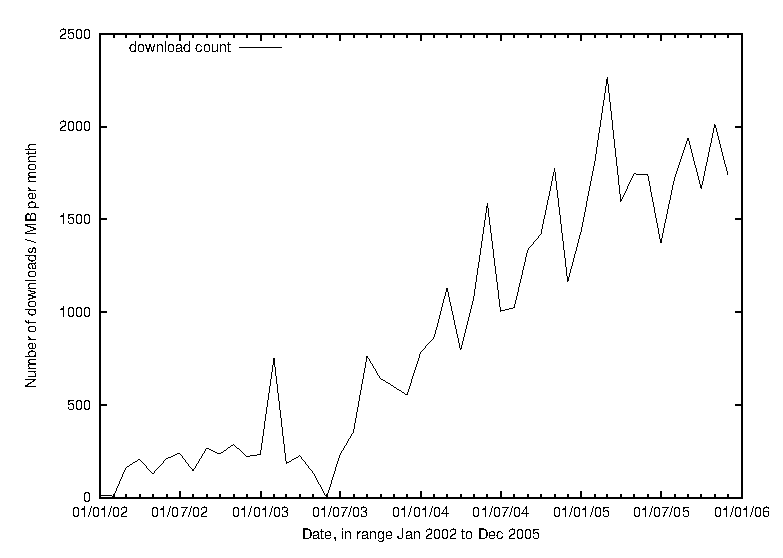
\includegraphics[width=\columnwidth]{ps_stats}
\caption{\label{32:fig-ps_downloads}Four-year download history for the Player/Stage Project}
\end{center}
\end{figure}

\begin{figure}[top]
\begin{center}
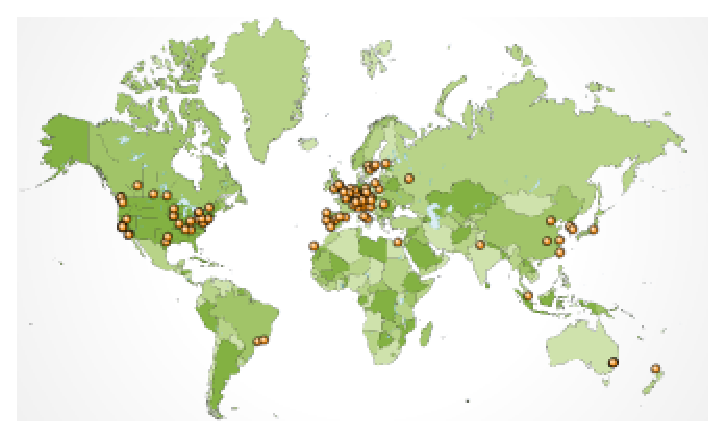
\includegraphics[width=\columnwidth]{ps_distribution}
\caption{\label{32:fig-ps_world}Geographical distribution of downloads in December 2005}
\end{center}
\end{figure}

Our claim that code from the Player/Stage Project is frequently reused
needs some supporting evidence. Player's distribution terms, the GNU
General Public License\footnote{\tt http://www.gnu.org/copyleft/gpl.html} allow anyone to use and distribute
the sourcecode. This makes it impossible to obtain precise numbers of
Player users. There is no reliable mechanism for user registration or
reporting. We have four sources of documentary evidence that Player
code is being used:

\begin{enumerate}
\item Download statistics;
\item Support forum messages and bug tracker items; 
\item Submissions to our user laboratory list; 
\item Acknowledgements in published robotics articles.
\end{enumerate}

The Player/Stage Project has been hosted by Sourceforge\footnote{\tt
http://sourceforge.net} since December 2001. As of 6 January 2006,
Sourceforge reported 42,009 downloads of P/S software, and a download
rate of around 2,000 packages (2.2GB) per month.


Figure \ref{32:fig-ps_downloads} is a graph of the number of downloads and
bandwidth supplied by Sourceforge each month of that four-year period
2001 through 2005. Downloads show faster-than-linear growth during
2002-4, and were roughly constant in 2005. No major new releases were
made in 2005: most development this year was towards a forthcoming 2.0
release scheduled for early 2006.

Google's web traffic analytics tracking service\footnote{\tt
http://google.com/analytics} provides (among other things) a
breakdown of the geographical location of visitors to the P/S web site. In
the month of December 2005, a total of 70,920 web page requests were
served. Figure
\ref{32:fig-ps_world} shows the locations of the visitors, 
demonstrating the global interest in Player. Unfortunately
geographical data for actual software downloads (rather than web page
requests) is not available, but we can assume that the distribution of
software downloads is similar to that of the web requests.

\subsection{Support forum and trackers} 

\begin{table}[top]
\begin{center}
\begin{tabular}{|l|l|r|r|}
\hline
{\bf Mailing list} & {\bf Description} & {\bf Subscribers} & {\bf Messages} \\ \hline
playerstage-users & Player and Stage user support & 253 & 3057 \\
playerstage-developers & developer discussion & 133 & 1423 \\
playerstage-gazebo & Gazebo user support & 99 & 864 \\
playerstage-design & strategic developer discussion & 58 & 130 \\ \hline
total messages & & & 5514 \\ \hline
\end{tabular}
\caption{\label{32:table-lists}Mailing list archive in January 2005}
\end{center}
\end{table}

\begin{table}[top]
\begin{center}
\begin{tabular}{|l|l|r|r|}
\hline
{\bf Tracker} & {\bf Items} \\ \hline
Bugs & 159 \\
Patches & 99 \\
Feature requests & 85 \\ \hline
total items & 243 \\ \hline
\end{tabular}
\caption{\label{32:table-trackers}Issue-tracking database items (including closed items) in January 2005}
\end{center}
\end{table}

P/S uses Sourceforge's mailing list and issue-tracker services to
communicate with users and developers. Activity on these services
suggests active users. Table \ref{32:table-lists} shows the number of
subscribers and messages on each list at the beginning of 2006.  There
were a total of 5514 messages on the lists since their creation
in January 2002; an average of three messages every day. The total
number of subscribers is not meaningful because many people subscribe
to more than one list.

Another indicator of user activity is the issue-tracking database, a
mechanism designed to manage issues that can not be immediately
resolved on the mailing lists. Figure \ref{32:table-trackers} shows
the number of items on each list from January 2001 to January 2006: a
total of 243. Notable here are the 99 code patches submitted by users
to fix bugs or extend P/S software. Many of these patches have been
applied to the tree to become `official' code.

\subsection{User site list}
Users are invited to submit the name of their laboratory for listing
on the P/S web site\footnote{\tt
http://playerstage.sourceforge.net/index.php?src=users} , which is
occasionally updated by the maintainers. The list currently contains
51 entries in 13 countries, including the Boeing Company, the
Australian Centre for Field Robotics, the Chinese National University
of Defense Technology, the Technical University of Munich, the NARA
Intitute of Science and Technology, Georgia Institute of Technology,
and Rochester Institute of Technology's DARPA Grand Challenge
Autonomous Race Team.

\subsection{References in scientific articles} 

Many authors not connected with P/S development or each other have
published papers that acknowledge the use of Player/Stage Project code
in their experiments. Examples include the papers
\cite{32_alankus05,32_haasch05,32_topp05,32_shao05} all 
from the IEEE International Conference on Intelligent Robots and
Systems (IROS) in 2005. Others are cited elsewhere in this chapter.

%\subsection{Other impact}
%Further anecdotal pieces of evidence a is that the developers are
%occasionally invited to speak about the project at international
%venues. The

%We do not have figures for other robot infrastructure projects for
%comparison. The most similar freely available system is CARMEN, the
%Carnegie Mellon Robot Navigation Toolkit, which is hosted at CMU and
%does not publicly provide download data. 

Based on these figures, we conclude that Player/Stage is both a
well-known and well-{\it used} source of robot code.

\section{Design of the Player robot device interface}
All work, including robotics research, is impacted by the tools that
are used. Good tools simplify common tasks, while bad tools complicate
them. The assumptions that are built into a set of tools bias the
researcher who uses them toward particular kinds of solutions.
%The availability of flexible, reliable, and reusable tools for robot
%programming is crucial for the research community.

Our design philosophy is heavily influenced by the operating systems
(OS) community, which has already solved many of the same problems
that we face in robotics research.  For example, the principle
function of an operating system is to hide the details of the
underlying hardware, which may vary from machine to machine.
Similarly, we want to hide the details of the underlying robot.  Just
as I expect my web browser to work with any mouse, I want my
navigation system to work with any robot.  Where OS programmers have
POSIX, we want a common development environment for robotic
applications.  Operating systems are equipped with standard tools for
using and inspecting the system, such as (in UNIX variants) {\bf top},
{\bf bash}, {\bf ls}, and {\bf X11}.  We desire a similar variety of
high-quality tools to support experimental robotics.

Operating systems also support virtually any programming language
and style.  They do this by allowing the low-level OS interface
(usually written in C) to be easily wrapped in other languages, and
by providing language-neutral interfaces (e.g., sockets, files) when
possible.  Importantly, no constraints or normative judgments are made
on how best to structure a program that uses the OS\@.  We take the same
approach in building robotics infrastructure.  Though not strictly part
of the OS, another key feature of modern development environments is the
availability of standard algorithms and related data structures, such
as {\bf qsort()}, TCP, and the C++ Standard Template Library.  We follow
this practice of incorporating polished versions of established algorithms
into the common code repository, so that each researcher need not
re-implement, for example, Monte Carlo localization.  Finally, an important
but often overlooked aspect of OS design is that access is provided at all
levels.  While most C programmers will manage memory allocation with the
library functions {\bf malloc()} and {\bf free()}, when necessary they can
dig deeper and invoke the system call {\bf brk()} directly.  We need
the same multi-level access for robots; while one researcher may be content
to command a robot with high-level ``goto'' commands, another will want to
directly control wheel velocities.

In summary, our approach to building tools for robotics research is to
extend useful abstractions from the OS up {\it just enough} to enable
robotic devices to be used as easily as normal computer devices such
as mice and printers. Like an OS, we aim to provide resources as
transparently as possible, extending and managing the hardware but
otherwise keeping out of the user's way.


\section{Abstractions}
%{\bf \small
%\begin{itemize}
%\item PADI : Syntax and semantics of messages that can be passed to
%or from interfaces; what it means for two devices to be functionally
%equivalent; driver + interface = device
%\item Player protocol : Message format (header structure, field ordering)
%and sequence (each request message gets a reply message, etc.)
%\item Transport : Bit-packing, message routing, addressing, resource
%discovery (e.g., TCP client/server with XDR-formatted messages, JINI with
%Java-serialized messages)
%\item Implementation : C++ Driver API, monolithic Linux-like device
%management, I/O multiplexing.
%\end{itemize}
%}
Player comprises four key abstractions: The Player Abstract Device
Interface (PADI), the message protocol, the transport mechanism, and
the implementation.  Each abstraction represents a reusable and
separable layer.  For example, the TCP client/server transport could
be replaced by a CORBA transport.  Alternatively, an entirely
different system could be built atop the PADI.  These four
abstractions, described in the following sections, are the result of a
considerable design effort refined over several years of broad use
and are in themselves opportunities for reuse, independent of their
P/S software implementations.


\subsection{The Player Abstract Device Interface}
%{\bf \small Borrow liberally from the ICAR paper (it's surprisingly well-written :).
%But remember that we've moved from a single-data/single-command
%state-reflection model to a more general message-passing model.  It can
%still be seen as an instance of the character device model; it's just that
%a device can produce or consume different kinds of messages. }

The central abstraction that enables portability and code re-use in
Player is the PADI specification. The PADI defines the syntax and
semantics of the data that is exchanged between the robot control code
and the robot hardware.  For ease of use, the PADI is currently
specified as a set of C message structures; the same information could
instead be written in an Interface Definition Language (IDL), such as
the one used in CORBA systems.

The PADI's set of abstract robot control interfaces constitutes a virtual
machine, a target platform for robot controllers that is instantiated at
run time by particular devices.  The goal of the PADI is to provide a
virtual machine that is rich enough to support any foreseeable robot control
system, but simple enough to allow for an efficient implementation on a
wide array of robot hardware.  The key concepts used in the PADI, both
borrowed from the OS community, are the character device model and the
driver/interface model.

\subsubsection{The character device model}
The ``device-as-file'' model, which originated in Multics
\cite{32_FeiertagOrganick71} and was popularized by UNIX
\cite{32_RitchieThompson74}, states that all I/O devices can be thought of as
data files. A distinction is made between sequential and random access
devices. Sequential devices such as terminals and tapes produce and consume
streams of data one byte after another, and are called {\em character
devices}, while random access devices such as disk drives can manipulate
chunks of data in arbitrary orders, usually through a cache, and are known
as {\em block devices}. The nature of sensors and actuators is to produce
and consume data in time-extended streams: they are character devices.

The standard interface to character devices is through five
well-defined operations. Access to devices is controlled by {\em open}
and {\em close} operations. Data is collected from the device by a
{\em read} operation, and sent to the device by a {\em write}
operation.  The asynchronous read and write are sufficient on their
own for many devices, but a third transfer mechanism, the {\em ioctl}
(input/output control) provides a synchronous request/reply channel,
typically to access data that is persistent rather than sequential,
such as setting and querying the configuration of the device. All five
operations will indicate error conditions if they fail.

Player uses the character device interface to access its hardware devices.
For example, to begin receiving sensor readings, the appropriate device is
first opened, after which data can be read from it.  Likewise to control
an actuator, the appropriate device is opened, after which commands can be
written to it.  An ioctl mechanism is used for device configuration and for
atomic test/set and read/clear operations required by some devices. For
reasons explained elsewhere~\cite{32_GerkeyVaughan01a,32_GerkeyVaughanHoward03},
Player does not currently implement exclusive access to devices, so
multiple modules can simultaneously control the same device.  We are
considering adding exclusive access modes, which would be analogous to
file-locking mechanisms in operating systems.

The character device model has some drawbacks. In particular, since there
is no interrupt mechanism, clients must poll devices to receive new data.
This is not the best approach for low-latency I/O with high-speed devices,
which are usually interrupt-driven.  Player was designed to support update
rates of the order of 5-100Hz, covering the majority of research robots.
This model is unlikely to suffice for devices that operate on the order of
1MHz. Also, the ioctl channel is often used in a way that breaks device
independence and reduces portability, as discussed below.

Apart from the assumption of sequential access (supplemented with the
ioctl), the character device abstraction is neutral with respect to
programming language and style. Almost every programming language supports
this model, and almost any robot control architecture can be (and likely
has been) implemented atop the generic read/write/ioctl interface.  This
model has successfully supported UNIX-like operating systems for decades,
and Player for years.  We suggest that the character device model is a
suitable foundation for a robot device control standard.

\subsubsection{The interface/driver model}
The character device model defines only the broadest semantics of its
three channels (roughly: input, output and configuration), but imposes
no other structure on the data streams. Each device could have its own
unique data format, requiring controller code to be written
specifically for each device. Another powerful abstraction, the {\em
interface/driver} model determines the content of these streams and
provides the device independence that is the key to portable code.

The interface/driver model groups devices by logical functionality, so
that devices which do approximately the same job appear identical from
the user's point of view. An {\em interface} is a specification for
the contents of the data stream, so an interface for a robotic
character device maps the input stream into sensor readings, output
stream into actuator commands, and ioctls into device
configurations. The code that implements the interface, converting
between a device's native formats and the interface's required formats
is called a {\em driver}. Drivers are usually specific to a particular
device, or a family of devices from the same vendor.

Code that is written to target the interface rather than any specific
device is said to be {\em device independent}. When multiple devices have
drivers that implement the same interface, the controlling code is portable
among those devices.

Many hardware devices have unique features that do not appear in the
standard interface. These features are accessed by device-specific ioctls,
while the read and write streams are generally device independent.
Interfaces should be designed to be sufficiently complete so as to not
require use of device-specific ioctls in normal operation, in order to
maintain device independence and portability.

There is not a one-to-one mapping between interface definitions and
physical hardware components. For example, the Pioneer's native P2OS
interface bundles odometry and sonar data into the same packet, but a
Player controller that only wants to log the robot's position does
not need the range data. For portability, Player separates the data
into two logical devices, decoupling the logical functionality from
the details of the Pioneer's implementation. The pioneer driver
controls one physical piece of hardware, the Pioneer microcontroller,
but implements two different devices: {\tt position2d} and {\tt sonar}.
These two devices can be opened, closed, and controlled independently,
relieving the user of the burden of remembering details about the
internals of the robot.

Since Player was initially designed as an interface to our Pioneer 2-DX
mobile robots, early versions of the server provided almost transparent
access to specific components and peripherals of the Pioneer as it was used
in the USC Robotics Lab.  For example, each data packet from the sonars
comprised 16 range readings, because the Pioneer has 16 sonar transducers.
Likewise, command packets to the wheel motors comprised two velocities,
because the Pioneer is a non-holonomic, differentially-driven robot.

This Pioneer-specific device model was extensible, but did not encourage
code reuse or portability.  When code was added to provide
access to a new device, that device presented a unique, device-specific
interface that required device-specific support in control programs.  As a
result, programs that controlled the second Player-supported mobile
robot, the RWI B21r, used an API that was completely different from that
used to control the Pioneer, despite the fact the two robots are
functionally similar.

In order to more conveniently support different devices, we introduced
the interface/driver distinction to Player. An interface, such as {\tt
sonar}, is a generic specification of the format for data, command,
and configuration interactions that a device allows.  A driver,
such as {\tt pioneer-sonar}, specifies how the low-level device
control will be carried out.  In general, more than one driver may
support a given interface; conversely, a given driver may support
multiple interfaces.  Thus we have extended to robot control the
device model that is used in most operating systems, where, for
example, a wide variety of joysticks all present the same ``joystick''
interface to the programmer.

As an example, consider the two drivers {\tt pioneer-position} and
{\tt rwi-position}, which control Pioneer mobile robots and RWI mobile
robots, respectively.  They both support the {\tt position2d} interface
and thus they both accept commands and generate data in the same
format, allowing a client program to treat them identically, ignoring
the details of the underlying hardware.  This model also allows us to
implement more sophisticated drivers that do not simply return sensor
data but rather filter or process it in some way.  Consider the {\tt
lasercspace} driver, which supports the {\tt laser} range-finder
interface.  Instead of returning the raw range values, this driver
modulates them according to the dimensions of the robot, creating the
configuration-space representation of free space in the environment.

The primary cost of adherence to a generic interface for an entire class
of devices is that the features and functionality that are unique to
each device are ignored.  Imagine a {\tt fiducial-finder} interface
whose data format includes only the bearing and distance to each
fiducial.  In order to support that interface, a driver that can also
determine a fiducial's identity will be under-utilized, some
of its functionality having been sacrificed for the sake of portability.
This issue is usually addressed by either adding configuration requests
to the existing interface or defining a new interface that exposes the
desired features of the device.  Consider Player's Monte-Carlo
localization driver {\bf amcl}; it can support both the sophisticated
{\tt localization} interface that includes multiple pose hypotheses,
and the simple {\tt position2d} interface that includes one pose and is
also used by robot odometry systems.

\subsection{The Player protocol}
%{\bf \small Brief explanation of the protocol, why it's simple,
%lightweight, and good for robots.}
The {\bf Player Protocol} implements the PADI along with some additional
structures and rules for multiplexing, ordering, sending and receiving
collections of PADI messages, and commands for inspecting and controlling
the behavior of Player itself.  For example, part of the protocol
specification states that data and messages are asynchronous and not
acknowledged, while configurations are synchronous: every request is
guaranteed an acknowledgment (positive or negative) in response.  The
protocol also defines a generic header structure that precedes every
message and contains the meta-data necessary to unambiguously interpret the
message.  Note the the protocol does not specify the manner in which
packets are serialized, addressed, or transmitted; those details are
handled by the transport layer.

\subsection{Transport mechanisms}
%{\bf \small Discussion of what it means to be transport-independent, both
%good and bad consequences.  E.g., you can pick JINI (or CORBA, etc.) if
%that's right for your application, but then you can't use existing
%TCP-based tools, like playernav.  Actually, I also exposed libplayertcp
%in the Java wrappers, so you can in fact run JINI and TCP in parallel
%(the main system uses JINI but I can poke in to debug via TCP), but
%the point is that in general you can't mix tools or systems that use
%different transports.}

The PADI and Player Protocol together are sufficient for building a
single-process robot control system.  Drivers can be instantiated and bound
to interfaces, and the resulting devices can exchange PADI-defined messages
(e.g., by function calls) according to the rules of the protocol.  However,
if we want the ability to move messages among devices or other modules that
are in different processes or on different machines, then we need a {\bf
transport} mechanism.\footnote{With respect to the OSI Network
Model~\cite{32_TannenbaumNetworks}, we refer collectively to the Network
Layers (Transport and below) and the packet-shuffling machinery in the
Session Layer as the {\em transport}.} The job of a transport mechanism is
two-fold: handle the addressing and routing of packets, and perform packet
serialization and deserialization (also called data marshaling).  Some
transports may also provide higher-level functionality, such as resource
discovery.

\subsubsection{TCP client/server transport}
Historically Player has relied on a TCP client/server transport, in which
devices reside in a {\em server} and a control program is a {\em client} to
the server.  To control a robot, the user first starts the {\bf player}
server, which listens on a particular TCP port (by default 6665), on the
robot.  Then a client program, such as a joystick controller or data
visualization GUI, is started and establishes a TCP socket connection to
the server.  The client can run on-board the robot or on any other machine
that has network connectivity to the robot.  One client can connect to many
servers and many clients can connect to one server.  Importantly, clients
can be written in any programming language with support for TCP sockets.

In order to safely send messages from one machine to another over a TCP
socket, a data marshaling scheme must be defined.  The marshaling rules
specify the bit-level details of how, for example, numbers are represented
on the wire.  Earlier versions of Player used a custom encoding of messages
as packed C structs that contained integers in network byte-order.   Player
now uses an open standard called eXternal Data Representation, or XDR
\cite{32_RFC1014}.  The XDR specifies an efficient, platform-independent
encoding for commonly-used data types, including integers and floating
point values.  To reduce the occurrence of marshaling bugs, the library that
performs the XDR data marshaling is generated in an automatic fashion
directly from the header file that specifies the PADI.

\subsubsection{Other transports}
The client/server model has served Player (and many other distributed
systems) well for many years, but it is not the ideal transport mechanism
for every robot system.  In order to allow for the use of other transports,
Player was redesigned to be transport-independent.  The TCP client/server
transport is still available (and will likely continue to be the mostly
widely-used), but other transport mechanisms can be substituted in its
place.  The drivers, message structures, and other underlying details
remain unchanged.

For example, we have developed a JINI-based transport for Player.  JINI is
a Java-based architecture for building distributed systems in a
network-centric manner \cite{32_Waldo99}.  JINI has been used in many
distributed systems, including the largest multi-robot system deployed to
date \cite{32_iser04}.  JINI offers a number of advantages over the TCP
client/server approach, including: robustness to network delays and
dropouts, automatic resource discovery, and effortless data marshaling
using Java's built-in object serialization mechanism.  On the other
hand, it is non-trivial to install, configure, and run the JINI
infrastructure; and of course control programs must be written in Java.

Other trade-offs exist for other popular transport mechanisms, such as
CORBA \cite{32_CORBA}, IPC \cite{32_IPC}, and ACE/TAO \cite{32_ACETAO}.  It
is highly unlikely that the robotics community will agree on a single
transport for all robotics software, nor should they; the requirements and
constraints exhibited by any given application area will make particular
transports more or less appropriate, and it is important to allow the
system designer to choose the best one.  Because the manual construction of
a new Player transport layer is a tedious and bug-prone process, we have
taken care with the the PADI and core Player libraries so as to facilitate
the automatic generation of transport code.  For example, the JINI
transport layer uses automatically-generated Java bindings for Player.  We
expect to see other transports developed similarly.

The choice of transport is critical for a robotics application as it
is the transport that determines the real-time peformance of the
system. Assuming that the robot software has been designed to avoid
any logically unecessary time delays, the transport and the underlying
OS that implements it are the only source of timing delays due to
buffering, message transmissionn, etc. For control of most
slow-moving, statically-stable wheeled robots, TCP over Ethernet (802.3) or
WiFi (802.11b/g) is found to have acceptable timing performance and its ubiquity
makes it a good choice of general purpose transport.

\subsection{Implementations}
%{\bf \small Overview of our implementation and why we did it that way.
%Alternative implementations might: be written in Java (e.g., for embedded
%platforms that natively execute Java); follow a microkernel Mach-like
%approach in which each device is managed in a separate process; not
%allow for multiple consumers of data from a device.  Of course you can't
%use the existing drivers, written in C/C++, in a native Java system.}

We have implemented the PADI, the Player Protocol, TCP client/server
transport (with XDR data marshaling), and many device drivers as a set
of reusable C/C++ libraries.  The most common use of these libraries
is in an executable server, called {\bf player}.  This server is used
to parse configuration files, instantiate drivers, and service client
connections to devices.  It is customary when using Player to assign
to each robot a server that contains all the drivers used in that
robot's control system.  The user's control program is written as a
client that executes outside of the server (the situation is
essentially the same, with different terminology, when using JINI
instead of TCP).

The server represents a privileged space in which modules have better,
faster access to hardware and to each other.  Control code on the client
side experiences greater latency and a somewhat lessened ability to
interrogate devices.  On the other hand, the client code has fewer
constraints with respect to programming language and structure, and it is
relieved of the drivers' burden of behaving properly to avoid crashing the
rest of the system.

In this way, Player is analogous to a monolithic kernel operating system,
in which a privileged kernel space is separated from a non-privileged user
space \cite{32_osbook}.  Most operating systems, including Linux, employ
monolithic kernels.  An alternative approach, used by operating systems
such as QnX, is the microkernel, in which there is no privileged kernel
space, but rather a collection of system processes and a mechanism for
efficiently passing messages between them.  There are advantages and
drawbacks to each approach and the topic has been debated, without
resolution, in the OS community for decades.  An example of a
microkernel-like robot control system is CARMEN \cite{32_Roy03IROS}.  It is
worth noting that although Player more naturally operates as a monolithic
kernel, a microkernel system can be constructed by connecting multiple
servers together, each with a single driver (server-server communication
operates exactly like client-server communication).

As an alternative to our C/C++ system, an equivalent implementation of
Player could be done in, for example, Java.  A Java-only Player would be
useful for the many embedded computing platforms that execute Java bytecode
natively.  Of course the existing C/C++ drivers could not be used on a
native Java system.  Other possible re-implementations include using
strictly C (for systems without C++ runtime support) and removing the
reliance on POSIX threads (which Player uses extensively).


\section{Higher-level drivers}
%The Player Driver API defines a standard way to implement such a module.
%Talk about Player acting as a community code repository, which allows
%the sharing, evaluation, and wider testing of implemented components.
%Having other people bang on your navigation system with their robot can
%only make your code better, right?}

While Player's primary purpose is to provide portable and nearly
transparent access to robot hardware, an increasing number of drivers
encapsulate sophisticated algorithms that are removed by one or more
steps from the physical hardware.  These {\em higher-level drivers}
use other drivers, instead of hardware, as sources of data and sinks
for commands.  The {\bf amcl} driver, for example, is an adaptive
Monte Carlo localization system \cite{32_ThrunFox03} that takes data
from a {\bf position2d} device, a {\bf laser} device, and a {\bf map}
device, and in turn provides robot pose estimates via the {\bf
localize} interface (as mentioned above, {\bf amcl} also supports the
simpler {\bf position2d} interface, through which only the most likely
pose estimate is provided).  Other Player drivers perform
functionality such as path-planning, obstacle avoidance, and various
image-processing tasks.

The development of such higher-level drivers and corresponding interfaces
yields three key benefits.  First, we save time and effort by implementing
well-known and useful algorithms in such a way that they are immediately
reusable by the entire community.  Just as C programmers can call
{\bf qsort()} instead of reimplementing quicksort, robotics students
and researchers students should be able to use Player's {\bf vfh}
driver instead of reimplementing the Vector Field Histogram navigation
algorithm \cite{32_vfh}.  The author of the driver benefits by having
her code tested by other scientists in environments and with robots to
which she may not have access, which can only improve the quality of the
algorithm and its implementation.  Second, we create a common development
environment for implementing such algorithms.  Player's C++ {\bf Driver}
API clearly defines the input/output and startup/shutdown functionality
that a driver must have.  Code that is written against this API can enter
a community repository where it is easily understood and can be reused,
either in whole or in part.  Finally, we create an environment in which
alternative algorithms can be easily substituted.  If a new localization
driver implements the familiar {\bf localize} interface, then it is a
drop-in replacement for Player's {\bf amcl}.  The two algorithms can be
run in parallel on the same data and the results objectively compared.

\section{APIs}

%%{\bf \small What it means to have an API for a robot.  Despite the
%%generality of Player, most users see only the libplayerc++ API, so for them
%%that's what's important.  We talked about this some in the ICAR paper.}

We have described above the various interfaces to Player's
components. In practice, the majority of user code will interact with
Player through a {\it client library}; a language-specific interface
that the user compiles (or loads, depending on the language) into
their client program. Each client library presents an `Application
Programming Interface' (API). The most commonly used client libraries
(and hence APIs) are the libplayerc and libplayerc++ libraries, for C
and C++ respectively. Several other libraries are thin wrappers around
one of these. For example the Python client library is automatically
generated from libplayerc using the SWIG (Simplifiedf Wrapper and
Interface Generator) tool \cite{32_swig}. Using SWIG, changes to the
libplayerc interface are correctly propogated through to APIs in
several languages without having to tediously edit each by hand. As
well as saving time, this removes a common source of bugs.

There are several advantages for users in using the client libraries
instead of talking to the Player server directly; first, client
libraries hide the details of the client/server communications almost
completely, so the user can largely ignore the socket-level Player
protocol, marshalling and serializing data, etc. Secondly, each API is
designed to in a way that is natural way for its language; for example
libplayerc++ presents client-side proxy objects that correspond to
server-side devices. Thus the user can manipulate the proxies as
fully-fledged objects, inherit from them, etc. As required by its
language, the C client library has a similar proxy-based design, but
structures and function calls are used instead.

Client library external APIs must change only when the PADI changes:
they need not change with the client/server protocol, though of course
the libraries must change internally to communicate with the
server. The APIs can often be backwards compatible, for example when
the PADI is extended but existing specifications are not changed the
client API will still work, it will simply not provide access to the
newly-defined structures.

As a `Presentation Layer' interface in OSI terms, the client library
APIs are almost independent of the transport layer in that they hide
most details of the transport. However, some high-level
transport-related details may leak through this abstraction. For
example, all the client libraries that target the Player TCP server
must be supplied with the hostname and port number of a running Player
server on initialization. After initialization, the TCP connection is
completely transparent as user code interacts with Player through
client-side proxy objects (C++, Java, Python) or structures and
function calls (C).

%In the past, some client libraries supported the Player UDP server,
%but this was found to be very little used, so UDP support has been
%removed since Player-2.0.

The popularity of the client libraries, particularly libplayerc++ and
libplayerc, means that their design is very important. As the
most-used interface anywhere in the Player/Stage system, the quality
of their design plays a large part in the utility of the whole
system. If the APIs are too complex, or inconsistent, or poorly
documented, users will be quickly frustrated. Libplayerc was carefully
designed to be as consistent and transparent as the authors could
reasonably make it. It was intended to replace libplayerc++ which was
written originally to test the Player TCP server and not intended for
end-users. The fact that almost all early users used the C++ library
instead of talking to the server took us by surprise.

For most users, the internal design of the server is of no interest at
all, so long as she is protected from it by a client library. However,
code correctness is equally important throughout the system: a bug
anywhere upstream will eventually appear to the user through this
interface. The existence of clean, maintainable server code is
justfied by the increased probability of code correctness alone. 

\section{Tools}

\begin{figure}[t]
\begin{center}
\subfigure[]{
  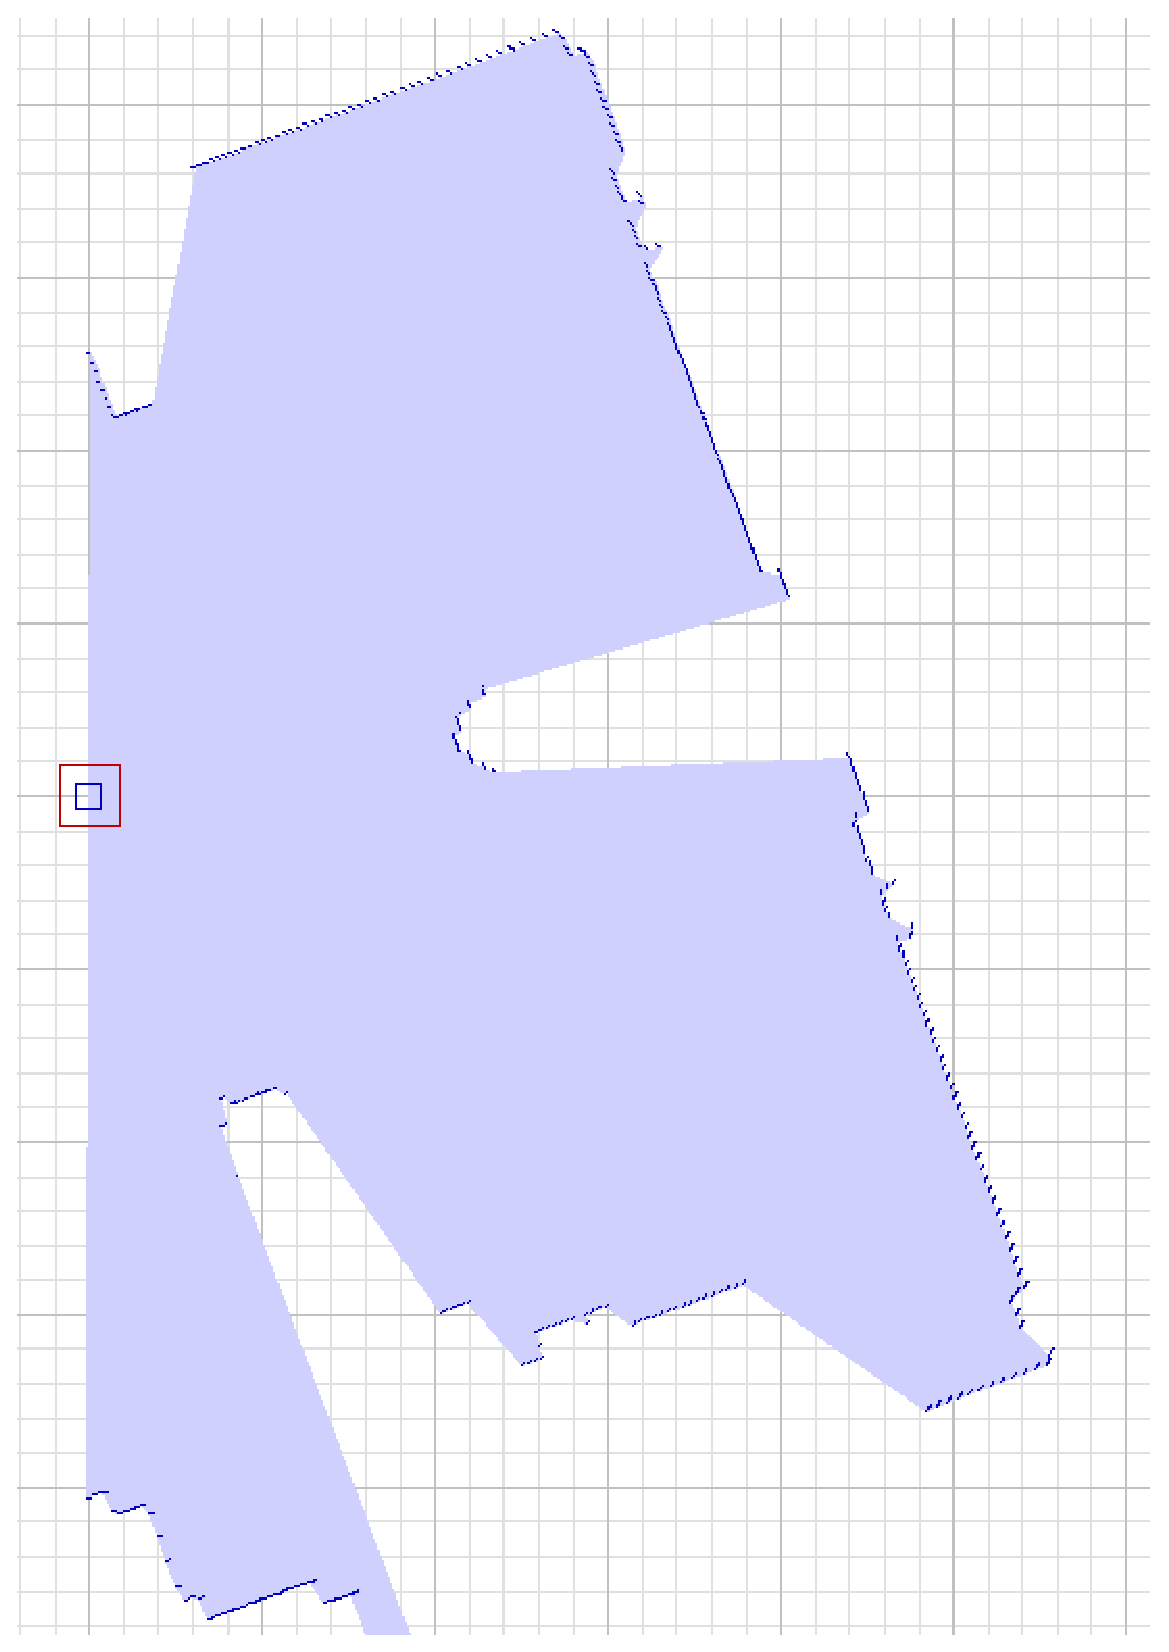
\includegraphics[width=.35\columnwidth]{playerv}
  \label{fig:ch32-playerv}
}
\subfigure[]{
  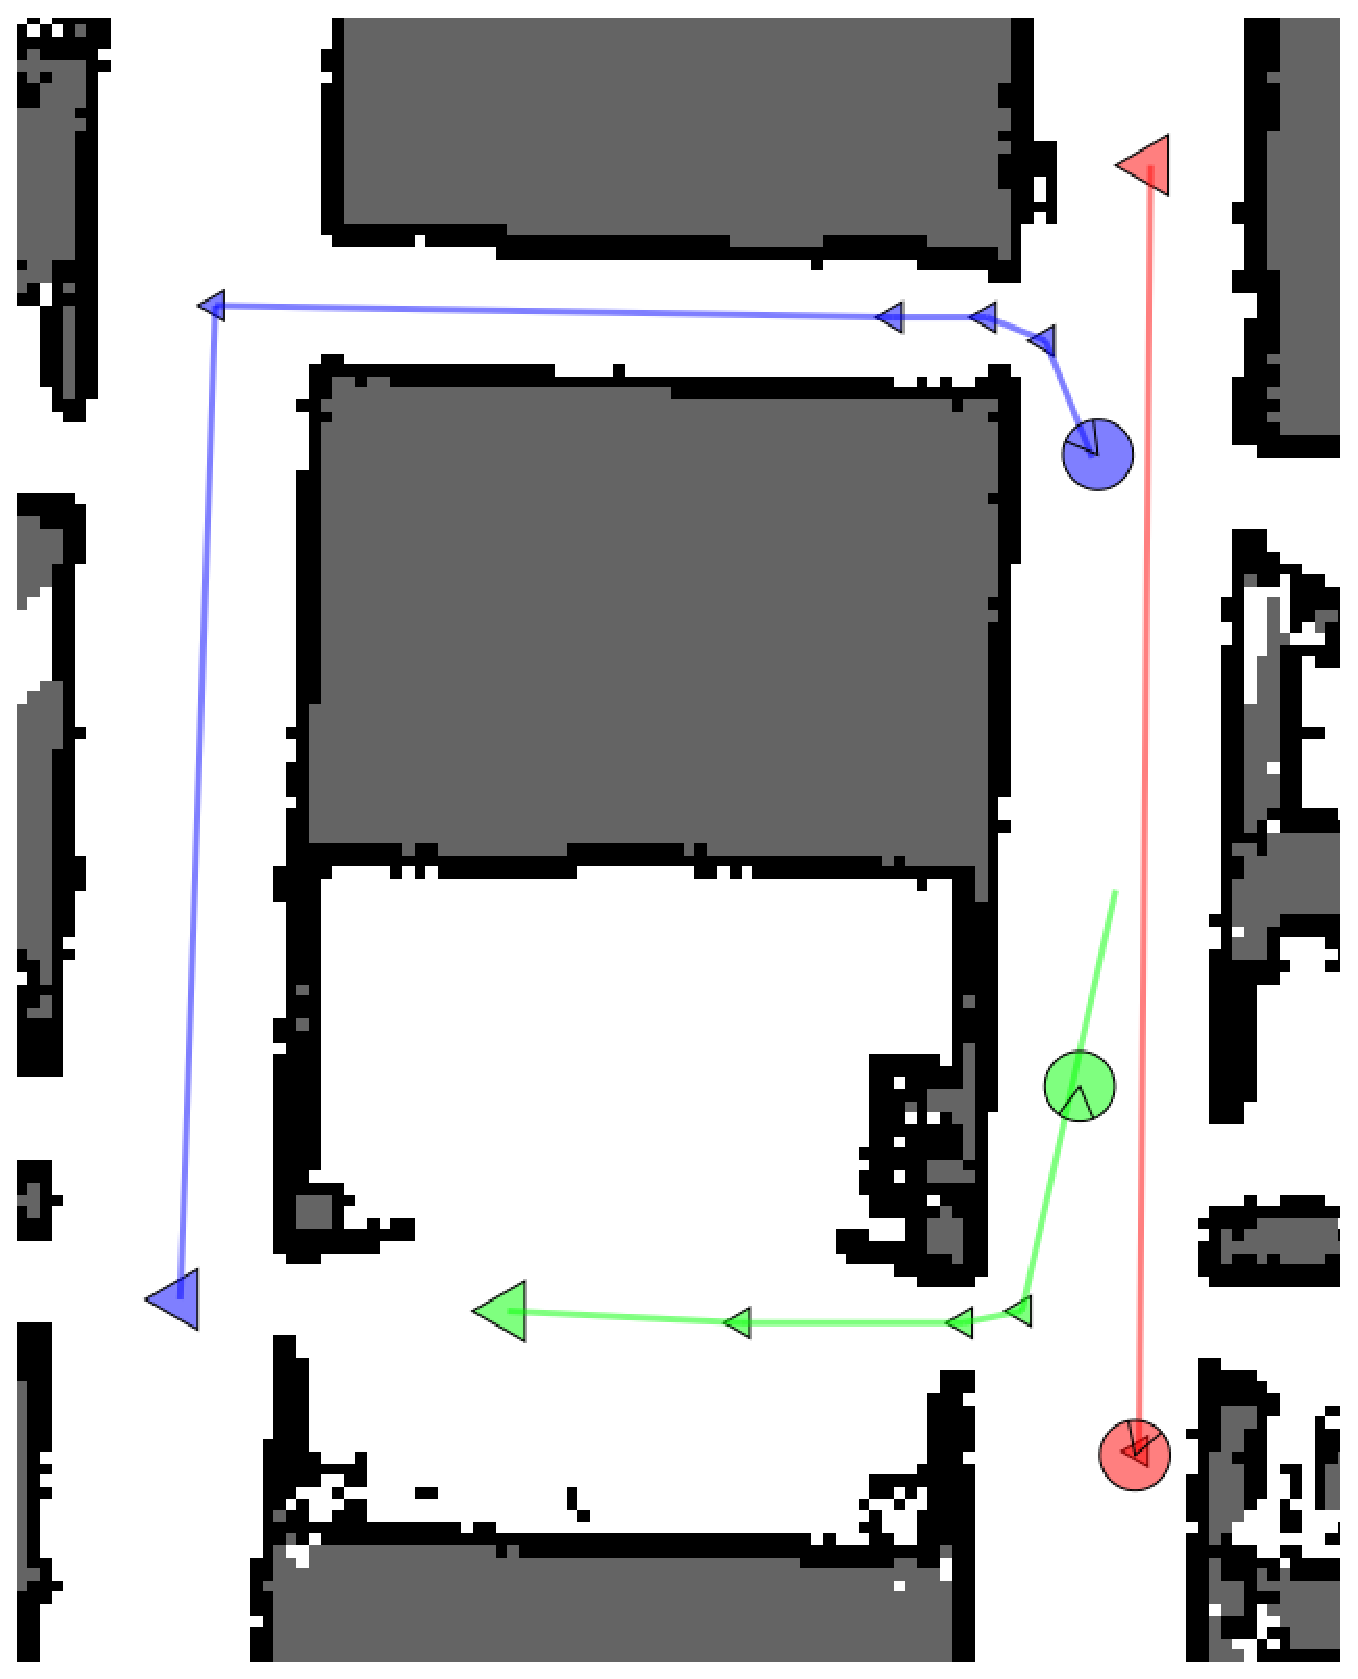
\includegraphics[width=.4\columnwidth]{playernav}
  \label{fig:ch32-playernav}
}
\caption{Screenshots of: (a) {\em playerv} displaying range data from
a laser-equipped robot; and (b) {\em playernav} showing poses and planned
paths for a team of robots.}
\end{center}
\end{figure}

As an OS provides the basic services needed to control a computer,
Player provides the basic services necessary to control a robot.
An OS is also bundled with useful tools for common tasks, like listing
files and displaying the process table.  Similarly, Player is bundled with
several tools:
\begin{itemize}
\item {\bf playerprint} : Fetches and prints sensor data to the console.
\item {\bf playerv} : Fetches and graphically displays sensor data; also
provides teleoperation by mouse movement (Figure~\ref{fig:ch32-playerv}).
\item {\bf playerjoy} : Provides joystick teleoperation.
\item {\bf playervcr} : Provides remote control of data logging and
playback.
\item {\bf playernav} : A graphical operator control unit that
provides control over localization and path-planning for multiple robots
(Figure~\ref{fig:ch32-playernav}).
\item {\bf playerwritemap} : Fetches grid and vector maps (e.g., from a
SLAM driver) and writes them to disk.
\item {\bf playercam} : Remotely displays video imagery from robot-mounted
cameras.
\end{itemize}
Third-party tools have also been developed, including a tool similar to
{\bf playercam} and an OpenGL-based 3-D application that combines some
of the functionality of {\bf playerv} with some of {\bf playernav}.
The development of such tools by users outside of the P/S/G project is
a testament to the reusability of the system and the extensibility of
the architecture.

\section{Simulation}

A significant contribution of the Player/Stage project is to provide
robot simulators. The main benefits to the user of using a simulation
over a real robot are convenience and cost: simulated robots are
usually easy to use, their batteries need not run out, and they are
very much cheaper than real robots.

\subsection{Stage}

After Player, the next most reused component of the Player/Stage
project is the Stage robot simulation engine. Stage provides a virtual
world populated by mobile robots and sensors, along with various
objects for the robots to sense and manipulate.  Designed with
multi-agent systems in mind, it provides fairly simple,
computationally cheap models of lots of devices rather than attempting
to emulate any device with great fidelity. This design is intended to
be useful compromise between conventional high-fidelity robot
simulations, the minimal simulations described by Jakobi
\cite{32_jakobi:ab}, and the grid-world simulations common in artificial
life research \cite{32_wilson:animat}. We intend Stage to be just realistic
enough to enable users to move controllers between Stage robots and
real robots, while still being fast enough to simulate large
populations. We also intend Stage to be comprehensible to
undergraduate students, yet sophisticated enough for professional
reseachers.

\begin{figure}[top]
\begin{center}
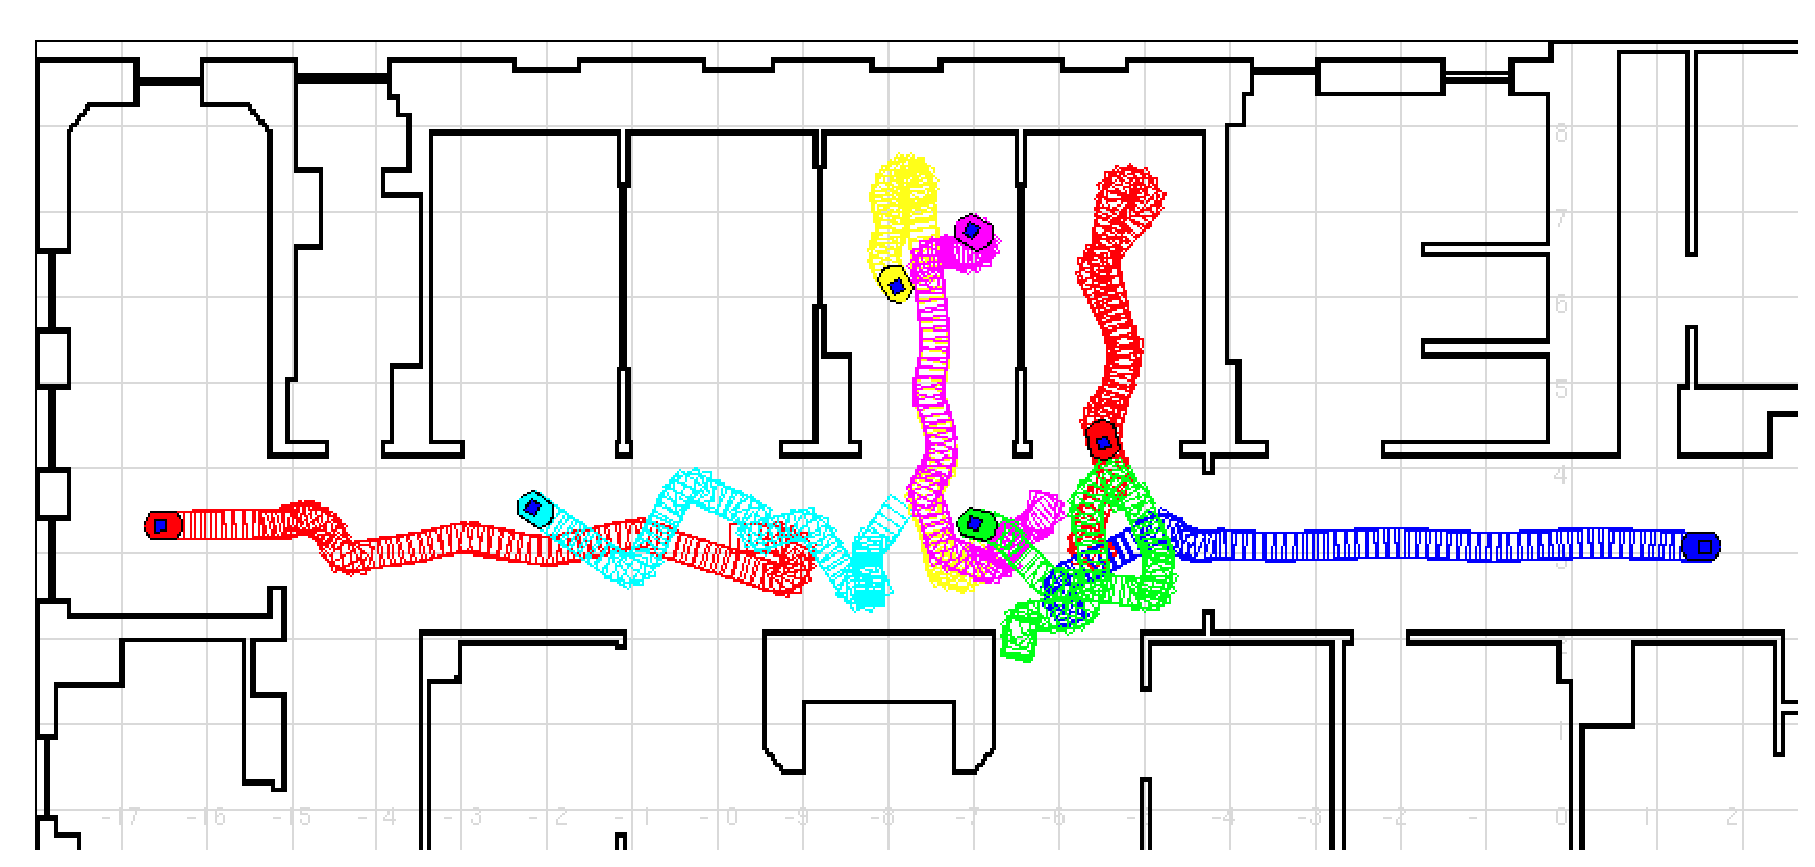
\includegraphics[width=\columnwidth]{ps_stage2}
\caption{\label{fig:ch32-stage}A screenshot from the Stage multiple-robot simulation, showing several robots leaving trails as they explore a small section of a hospital floorplan.}
\end{center}
\end{figure}


\begin{figure}[top]
\begin{center}
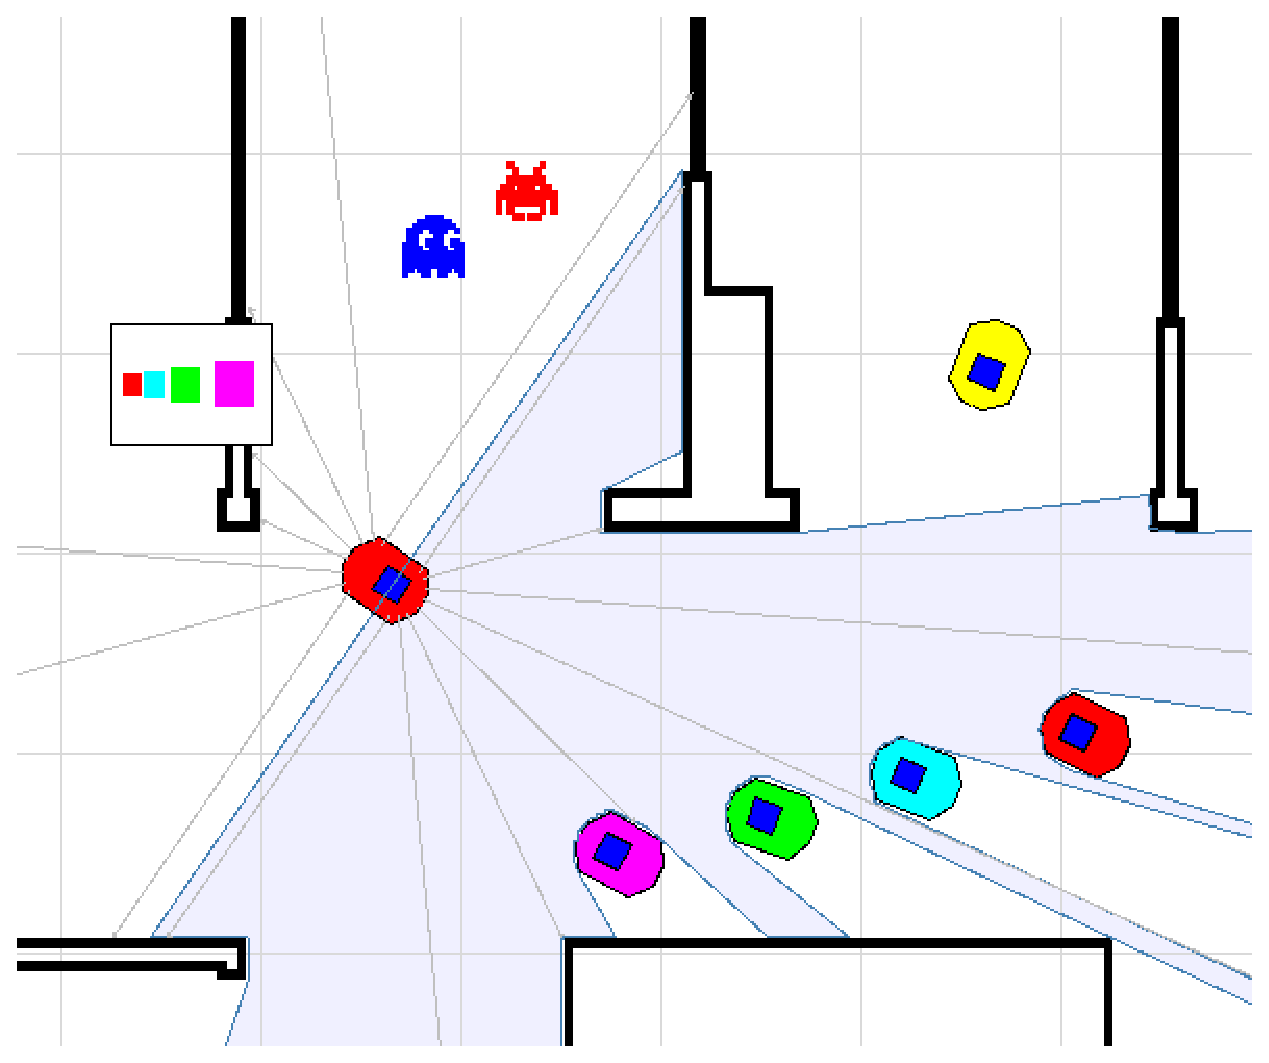
\includegraphics[width=80mm]{ps_stage}
\caption{\label{fig:ch32-stage2}A close-up screenshot from the Stage multiple-robot simulation, showing rendered laser and sonar data and several robots.}
\end{center}
\end{figure}

Stage provides several sensor and actuator models, including sonar or
infrared rangers, scanning laser rangefinder, color-blob tracking,
fiducial tracking and mobile robot bases with odometric or global
localization. Figures \ref{fig:ch32-stage} and \ref{fig:ch32-stage2} show
screenshots from a running simulation.

Stage is most commonly used with Player to form the Player/Stage
system. Robot controller client programs interact only with Player, so
simulated Stage devices appear identical to real devices. Client
programs do not need to be rewritten or even recompiled to switch from
simulated to real devices: a very convenient feature. Stage is
implemented as a Player plugin driver ({\tt libstageplugin}), loaded
as Player starts up. This allows Stage to be developed and released on
a schedule independent of Player.


\begin{figure}
\begin{center}
\begin{verbatim}
#include "stage.h"

int main( int argc, char* argv[] )
{ 
  stg_init( argc, argv );
  stg_world_t* world = stg_world_create_from_file( argv[1] );
  
  while( (stg_world_update( world,TRUE )==0) )
    {
      /* use the simulation */
    }
 
  stg_world_destroy( world );
  return 0;
}
\end{verbatim}
\caption{\label{fig:ch32-libstage}Creating a complete multiple-robot simulation in C with libstage.}
\end{center}
\end{figure}


The Stage simulation engine is implemented as the standalone C library
{\tt libstage}; libstageplugin is a wrapper around libstage that
connects it to Player's driver architecture. Libstage can be used to
very easily create a robot simulation in user code. This is useful for
users who wish to have more control over the internals of a simulation
than they can get through Player's {\tt simulation} interface. It also
allows for perfectly repeatable experiments, without the unpredictable
timing inevitably introduced by Player's TCP transport. 

Using Stage directly without Player also saves a little computational
overhead for those with very high performance requirements. The main
downside is the loss of Player's high-level drivers (VFH, AMCL,
etc.). Using the libstage in this way is very simple, as illustrated
Figure
\ref{fig:ch32-libstage} showing the C code required to instantiate a
complete multiple robot simulator, similar to that shown in the
screenshot above.

Stage is probably the most-used robot simulator, with research papers
acknowledging the use of Player/Stage appearing in most major journals
and conferences. The first published paper to use libstage directly
was \cite{32_Zhang06}, but libstage has also the basis of a the
commercial product ``MobileSim'' from MobileRobots Inc. since
2005. This is noteworthy because none of the Stage maintainers have
any relationship with the company or MobileSim, but MobileRobots have
been active in contributing patches back to libstage.

\subsection{Gazebo}

\begin{figure}[top]
\begin{center}
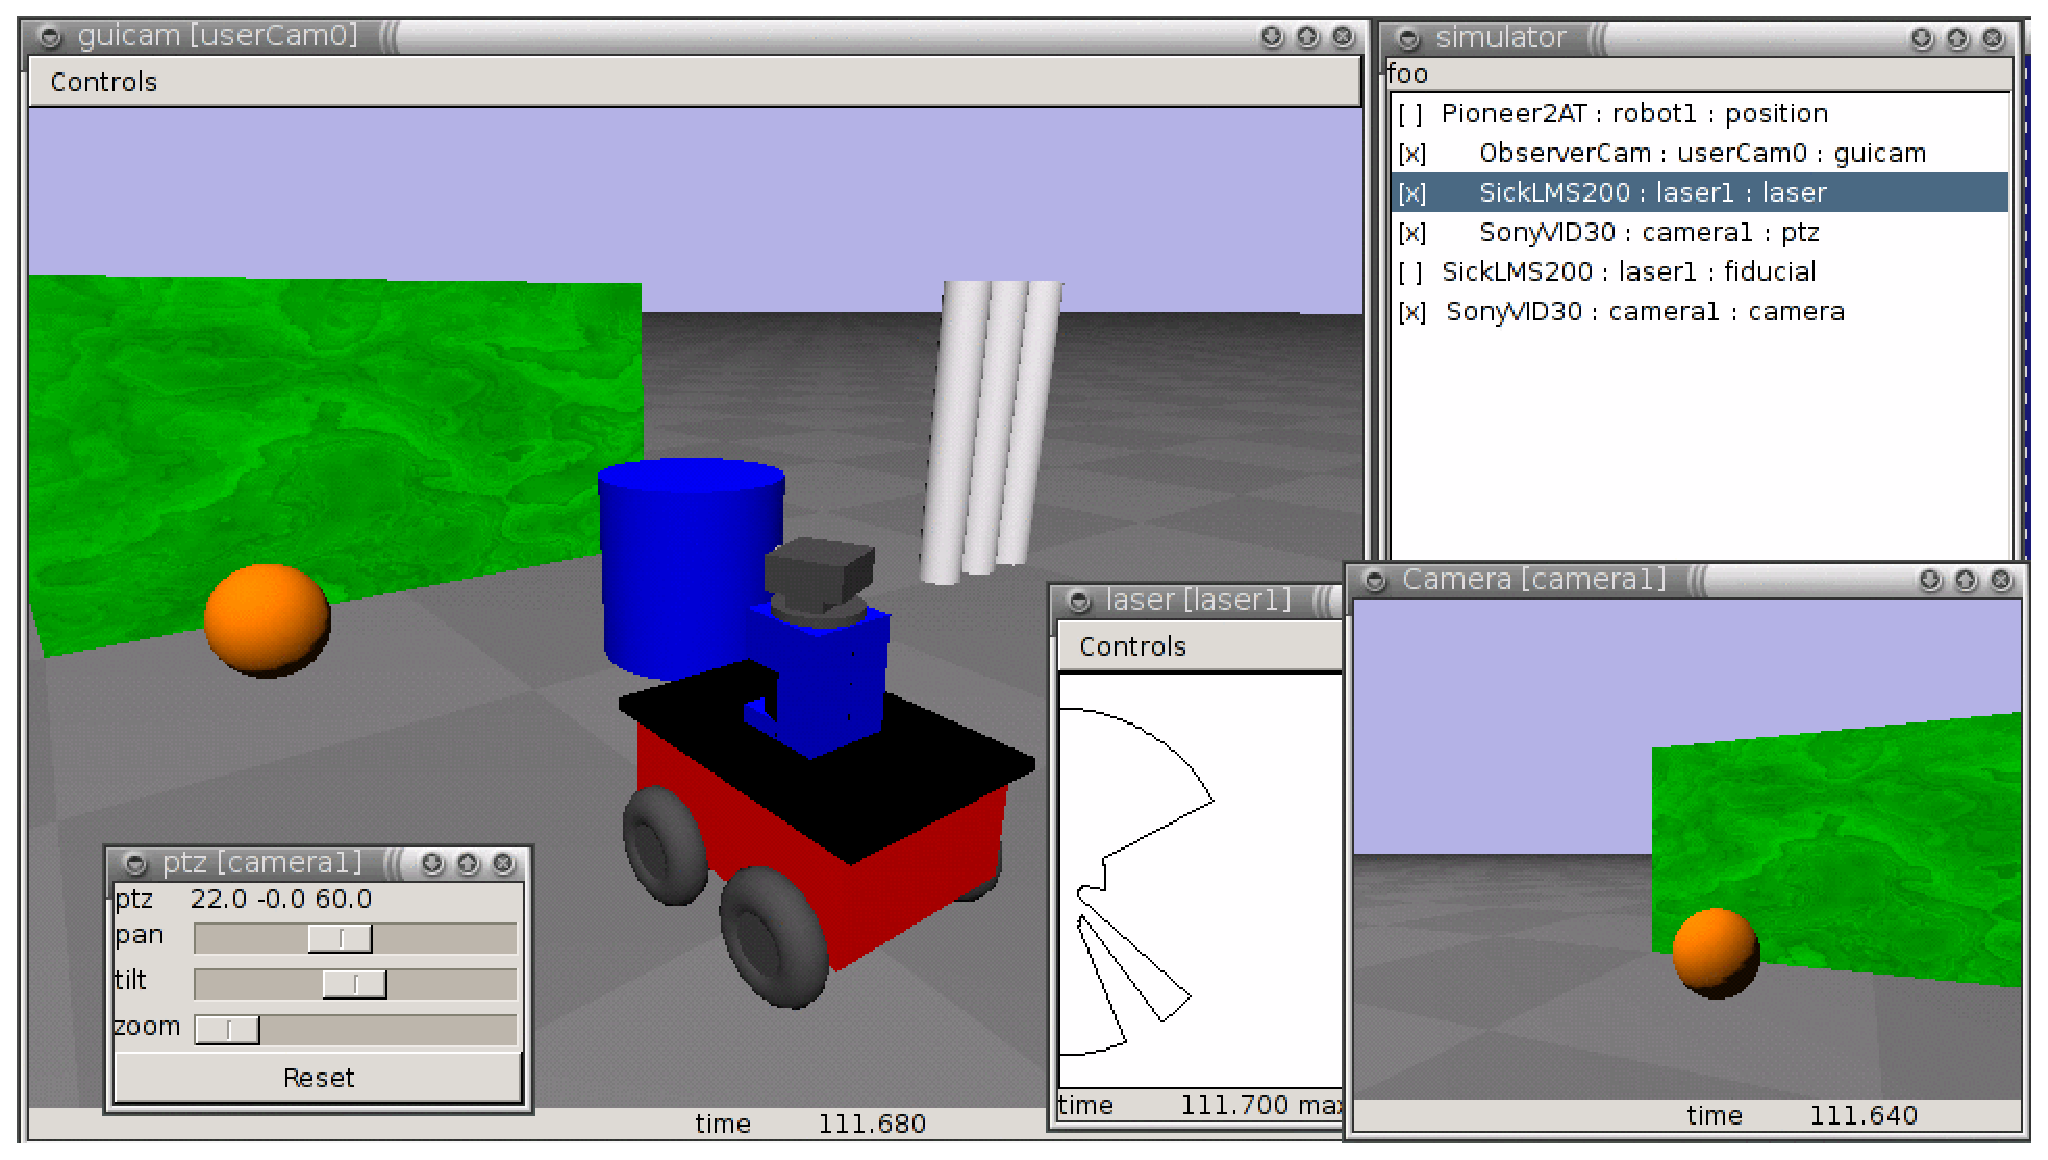
\includegraphics[width=\columnwidth]{ps_gazebo}
\caption{\label{fig:ch32-gazebo}A screenshot from the Gazebo 3D robot simulator,
 showing a model of a Pioneer robot carrying a SICK laser scanner and
 pan/tilt/zoom camera, with some environmental objects.}
\end{center}
\end{figure}

Gazebo is also a robot simulator that works with Player. Unlike Stage,
it provides realistic kinematics and dynamics in three-dimensional
environments. Figure \ref{fig:ch32-gazebo} shows a screenshot from
Gazebo. Client programs written using one simulator can usually be run
on the other with little or no modification. Gazebo is more realistic
than Stage, but much more computationally intensive. Stage is designed
to simulate a large robot population with low fidelity, and Gazebo is
designed to simulated a fairly small population with high
fidelity. Thus the two simulators are complimentary, and users may
switch between them without cost due to the common Player interface.

Like Stage, Gazebo is implemented as a standalone library and can be
used without Player. Due to its complexity, Gazebo is currently more
difficult to install and run than Stage, and is less frequently used.


\section{Barriers to reuse}

Why are most robot code tools used by no one but their authors? Robot
infrastructure code will not be widely used if it is

\begin{enumerate}
\item very buggy, or otherwise of poor quality;
\item undocumented;
\item too expensive;
\item tied to a specific robot platform.
\item not solving the problems that lots of people really have;
\item difficult for the user to express their intentions;
\item overwhelmingly complex or cumbersome to use;
\item not distributed.
\end{enumerate}

The first three reasons are self-explanatory, but the others may
require some elaboration.

Several well-known pieces of software are produced and/or distributed
by robot manufacturers to add value to their products. They
deliberately only work with that company's robots. The market for
robots is small and diverse, and many robots are still
custom-built. Robot companies often (perhaps usually?) go out of
business. When evaluating the software from a vendor, the researcher
has to decide if the software is worth the investment in time and
money (if the software is not free) to invest in software that
restricts her choice of robot, and for which the support from someone
with access to sourcecode could disappear at any time. These problems
are the same with all commmercial software, but the small size and
volatility of the research robot business makes this particularly
risky.

The next two reasons are closely related. Producing software that does
not solve anyone's real problems is a trap that is often fallen in
to. For example, one feature that is repeatedly proposed to make robot
programming easier is graphical programming, i.e. building systems by
connecting boxes with lines using some spatial layout tool. This seems
to ignore the fact that the population of robot programmers are
overwhelmingly graduates of computer science or engineering, most of
whom have no difficulty expressing themselves in code. Being
artificially constrained to thinking about a problem {\it only}
graphically, can be frustrating. Some common code structures, such as
loops and recursion, are difficult to represent graphically. As anyone
who has used Simulink knows, complex programs quickly lead to
cluttered screens and so lots of time is spent arranging objects
spatially: an arrangement that has no meaning at all for the
code. Great complexity is also a problem: users are quick to abandon a
system if they feel overwhelmed or can not get their robot equivalent
of ``Hello World'' working in a few hours.

Another problem is of overwhelmingly complex or cumbersome
software. Many of the proposed solutions to robot programming problems
require infrastructure that may take more time to install and debug
than they can save. The application of middleware such as CORBA, TAO
and JINI, attractive though it is to software engineers, must be
carefully justified to a robot programmer on a tight time budget, with
no one in the lab with past experience in these systems. Even
world-famous laboratories have ``rapid'' robot development systems
that are so complex that the in-bouse engineers will not use them for
real projects.

The final, and very basic reason that many systems are not widely used
is that they are not distributed. This is usually due to institutional
rules that prevent code from being given away free. The robot software
market is very small and few people will pay to license software, so
it stays within its development team only.

Notice that of these eight reasons, only the first two would
automatically be addressed by conventional software engineering
techniques. The rest are strategic, marketing and political problems
that can not be solved by applying object-oriented techniques or
client-server, publish-subscribe design patterns.

\section{Conclusion}

The most obvious way is to use code from the Player/Stage Project is
to use the software packages as distributed. We have presented
evidence above that this is happening frequently. However, the
resources developed in and around the Player/Stage Project can be
re-used in several different ways:

\begin{enumerate}
\item use the software packages as provided;
\item extend Player with new drivers and/or interfaces;
\item extend Stage or Gazebo with new simulation models;
\item use the simulation, driver or server libraries as part of custom software;
\item use the interface specification (PADI) as is, or as a guideline for creating custom interfaces
\item use the non-code resources, such as the Stage environment bitmaps that have become well-known;
\item use Player as middleware
\end{enumerate}

This last option will become important in the near future. The
drivers, PADI and Player Protocol specifications in Player are very
valuable resources. Player's strength is the transparency it provides
by trying to avoid placing constraints on the robot programmer. A
Player-equipped robot is a blank slate, with a loose collection of
easily accessible, commonly-used devices. A very suitable use for
Player is as a substrate, or middleware layer, for more structured
robot programming frameworks. If such a framework targetted Player
instead of robot hardware directly, it would automatically inherit the
large base of supported robots and implemented algorithms, saving the
authors a great deal of development time.

Code has a good chance of being widely reused if it is

\begin{enumerate}
\item solving a user's problems
\item supported by their robots, or easy to port;
\item easy enough to use;
\item easy to obtain;
\item good enough quality;
\item well documented;
\item affordable;
\item supported by a knowledgable group of people;
\end{enumerate}

We believe that Player/Stage is popular and widely used because it
meets these criteria better than any other current system. It is not
perfect, it is not finished, and it is not the right choice for every
application. It is the product of a community of robot programmers,
and it works for us.





%%%%%%%%%%%%%%%%%%%%%%%%%%%%%%%%%%%%%%%%%%%%%%%%%%%%%%%%%%%%%%%%%%%%%%
%\printindex %\end{document}

%%%%%%%%%%%%%%%%%%%%%%%%%% author.tex %%%%%%%%%%%%%%%%%%%%%%%%%
%
% sample root file for your contribution to a
%
% "contributed book" (global)
%
% Use this file as a template for your own input.
%
%%%%%%%%%%%%%%%%%%%%%%%% Springer-Verlag %%%%%%%%%%%%%%%%%%%%%%%%%%


%%% The following preamble of the contribution has been commented out
%%% to allow LaTeX to \include that document into the main book

% RECOMMENDED %%%%%%%%%%%%%%%%%%%%%%%%%%%%%%%%%%%%%%%%%%%%%%%%%%%
%\documentclass{svmult}

%% choose options for [] as required from the list
%% in the Reference Guide, Sect. 2.2

%\usepackage{makeidx}         % allows index generation
%\usepackage{graphicx}        % standard LaTeX graphics tool
                              % when including figure files
%\usepackage{multicol}        % used for the two-column index
%\usepackage[bottom]{footmisc}% places footnotes at page bottom
% etc.
% see the list of further useful packages
% in the Reference Guide, Sects. 2.3, 3.1-3.3

%\makeindex             % used for the subject index
                       % please use the style sprmidx.sty with
                       % your makeindex program


%%%%%%%%%%%%%%%%%%%%%%%%%%%%%%%%%%%%%%%%%%%%%%%%%%%%%%%%%%%%%%%%%%%%%

%\begin{document}

\title*{An Integration Framework for Developing Interactive Robots}
% Use \titlerunning{Short Title} for an abbreviated version of
% your contribution title if the original one is too long
\author{J. Fritsch\inst{1}\and S. Wredea\inst{1}}
% Use \authorrunning{Short Title} for an abbreviated version of
% your contribution title if the original one is too long
\institute{Bielefeld University, Faculty of Technology,, Germany
\texttt{\{fjannik,swredeg\}@techfak.uni-bielefeld.de}}
%
% Use the package "url.sty" to avoid
% problems with special characters
% used in your e-mail or web address
%
\maketitle

\section{Introduction}
\label{sec:ch33-Intro}

Text \cite{33_castek00component}.


\subsection{Subsection}
\label{sec:ch33-subsection}

Text


%%%%%%%%%%%%%%%%%%%%%%%%%%%%%%%%%%%%%%%%%%%%%%%%%%%%%%%%%%%%%%%%%%%%%%

%\printindex
%\end{document}

%%%%%%%%%%%%%%%%%%%%%%%%%% author.tex %%%%%%%%%%%%%%%%%%%%%%%%%
%
% sample root file for your contribution to a
%
% "contributed book" (global)
%
% Use this file as a template for your own input.
%
%%%%%%%%%%%%%%%%%%%%%%%% Springer-Verlag %%%%%%%%%%%%%%%%%%%%%%%%%%


%%% The following preamble of the contribution has been commented out
%%% to allow LaTeX to \include that document into the main book

% RECOMMENDED %%%%%%%%%%%%%%%%%%%%%%%%%%%%%%%%%%%%%%%%%%%%%%%%%%%
%\documentclass{svmult}

%% choose options for [] as required from the list
%% in the Reference Guide, Sect. 2.2

%\usepackage{makeidx}         % allows index generation
%\usepackage{graphicx}        % standard LaTeX graphics tool
                              % when including figure files
%\usepackage{multicol}        % used for the two-column index
%\usepackage[bottom]{footmisc}% places footnotes at page bottom
% etc.
% see the list of further useful packages
% in the Reference Guide, Sects. 2.3, 3.1-3.3

%\makeindex             % used for the subject index
                       % please use the style sprmidx.sty with
                       % your makeindex program


%%%%%%%%%%%%%%%%%%%%%%%%%%%%%%%%%%%%%%%%%%%%%%%%%%%%%%%%%%%%%%%%%%%%%

%\begin{document}

\title*{Increasing decoupling in a framework for programming robots}
% Use \titlerunning{Short Title} for an abbreviated version of
% your contribution title if the original one is too long
\author{Vincenzo Ambriola\inst{1}\and Antonio Cisternino\inst{1}\and
Diego Colombo\inst{2} \and Marco Combetto \inst{3}}
% Use \authorrunning{Short Title} for an abbreviated version of
% your contribution title if the original one is too long
\institute{University of Pisa, Computer Science Department, Pisa,
Italy \texttt{\{ambriola, cisterni\}@di.unipi.it} \and IMT Alti
Studi Lucca, Lucca, Italy \texttt{diego.colombo@imtlucca.it} \and
Microsoft Research ltd., Cambridge, United Kingdom,
\texttt{marcomb@microsoft.com} }
%
% Use the package "url.sty" to avoid
% problems with special characters
% used in your e-mail or web address
%
\maketitle

\section{Introduction}
\label{sec:ch34-Intro}

Text \cite{34_castek00component}.

\subsection{Subsection}
\label{sec:ch34-subsection}

Text

%%%%%%%%%%%%%%%%%%%%%%%%%%%%%%%%%%%%%%%%%%%%%%%%%%%%%%%%%%%%%%%%%%%%%%

%\printindex
%\end{document}

%%%%%%%%%%%%%%%%%%%%%%%%%% author.tex %%%%%%%%%%%%%%%%%%%%%%%%%
%
% sample root file for your contribution to a
%
% "contributed book" (global)
%
% Use this file as a template for your own input.
%
%%%%%%%%%%%%%%%%%%%%%%%% Springer-Verlag %%%%%%%%%%%%%%%%%%%%%%%%%%


%%% The following preamble of the contribution has been commented out
%%% to allow LaTeX to \include that document into the main book

% RECOMMENDED %%%%%%%%%%%%%%%%%%%%%%%%%%%%%%%%%%%%%%%%%%%%%%%%%%%
%\documentclass{svmult}

%% choose options for [] as required from the list
%% in the Reference Guide, Sect. 2.2

%\usepackage{makeidx}         % allows index generation
%\usepackage{graphicx}        % standard LaTeX graphics tool
                              % when including figure files
%\usepackage{multicol}        % used for the two-column index
%\usepackage[bottom]{footmisc}% places footnotes at page bottom
% etc.
% see the list of further useful packages
% in the Reference Guide, Sects. 2.3, 3.1-3.3

%\makeindex             % used for the subject index
                       % please use the style sprmidx.sty with
                       % your makeindex program


%%%%%%%%%%%%%%%%%%%%%%%%%%%%%%%%%%%%%%%%%%%%%%%%%%%%%%%%%%%%%%%%%%%%%

%\begin{document}

\title*{VIP - A Framework for Robot Vision based on MIRO}
% Use \titlerunning{Short Title} for an abbreviated version of
% your contribution title if the original one is too long
\author{Hans Utz\inst{1}\and Ulrich Kaufmann\inst{2}
\and Gerd Mayer\inst{2} \and Gerhard K. Kraetzschmar \inst{3}}
% Use \authorrunning{Short Title} for an abbreviated version of
% your contribution title if the original one is too long
\institute{AAA \texttt{aaa@aaa} \and University of Ulm,
Neuroinformatics, Ulm, Germany \texttt{\{kaufmann,
mayer\}@informatik.uni-ulm.de} \and Fraunhofer AIS, Sankt
Augustin, Germany \texttt{gerhard.kraetzschmar@ais.fraunhofer.de}}
%
% Use the package "url.sty" to avoid
% problems with special characters
% used in your e-mail or web address
%
\maketitle

\section{Introduction}
\label{sec:ch35-Intro}

Text \cite{35_castek00component}.


\subsection{Subsection}
\label{sec:ch35-subsection}

Text



%\printindex
%\end{document}

%%%%%%%%%%%%%%%%%%%%%%%%%% author.tex %%%%%%%%%%%%%%%%%%%%%%%%%
%
% sample root file for your contribution to a
%
% "contributed book" (global)
%
% Use this file as a template for your own input.
%
%%%%%%%%%%%%%%%%%%%%%%%% Springer-Verlag %%%%%%%%%%%%%%%%%%%%%%%%%%


%%% The following preamble of the contribution has been commented out
%%% to allow LaTeX to \include that document into the main book

% RECOMMENDED %%%%%%%%%%%%%%%%%%%%%%%%%%%%%%%%%%%%%%%%%%%%%%%%%%%
%\documentclass{svmult}

%% choose options for [] as required from the list
%% in the Reference Guide, Sect. 2.2

%\usepackage{makeidx}         % allows index generation
%\usepackage{graphicx}        % standard LaTeX graphics tool
                              % when including figure files
%\usepackage{multicol}        % used for the two-column index
%\usepackage[bottom]{footmisc}% places footnotes at page bottom
% etc.
% see the list of further useful packages
% in the Reference Guide, Sects. 2.3, 3.1-3.3

%\makeindex             % used for the subject index
                       % please use the style sprmidx.sty with
                       % your makeindex program


%%%%%%%%%%%%%%%%%%%%%%%%%%%%%%%%%%%%%%%%%%%%%%%%%%%%%%%%%%%%%%%%%%%%%

%\begin{document}

\title*{Using MARIE in Software Development and Integration for
Autonomous Mobile Robotics}
% Use \titlerunning{Short Title} for an abbreviated version of
% your contribution title if the original one is too long
\author{Carle C�t�\and Yannick Brosseau \and Dominic L�tourneau
\and Cl�ment Ra�evsky \and Fran�ois Michaud\inst{1}}
% Use \authorrunning{Short Title} for an abbreviated version of
% your contribution title if the original one is too long
\institute{Universit� de Sherbrooke,Department of Electrical
Engineering and Computer Engineering, Sherbrooke (Qu�bec), CANADA
\texttt{\{Carle.Cote, Yannick.Brosseau, Dominic.Letourneau,
Clement.Raievsky, Francois.Michaud\}@USherbrooke.ca}}
%
% Use the package "url.sty" to avoid
% problems with special characters
% used in your e-mail or web address
%
\maketitle

\section{Introduction}
\label{sec:ch36-Intro}

Text \cite{36_castek00component}.


\subsection{Subsection}
\label{sec:ch36-subsection}

Text


%%%%%%%%%%%%%%%%%%%%%%%%%%%%%%%%%%%%%%%%%%%%%%%%%%%%%%%%%%%%%%%%%%%%%%

%\printindex
%\end{document}

%%%%%%%%%%%%%%%%%%%%%%%%%% author.tex %%%%%%%%%%%%%%%%%%%%%%%%%
%
% sample root file for your contribution to a
%
% "contributed book" (global)
%
% Use this file as a template for your own input.
%
%%%%%%%%%%%%%%%%%%%%%%%% Springer-Verlag %%%%%%%%%%%%%%%%%%%%%%%%%%


%%% The following preamble of the contribution has been commented out
%%% to allow LaTeX to \include that document into the main book

% RECOMMENDED %%%%%%%%%%%%%%%%%%%%%%%%%%%%%%%%%%%%%%%%%%%%%%%%%%%
%\documentclass{svmult}

%% choose options for [] as required from the list
%% in the Reference Guide, Sect. 2.2

%\usepackage{makeidx}         % allows index generation
%\usepackage{graphicx}        % standard LaTeX graphics tool
                              % when including figure files
%\usepackage{multicol}        % used for the two-column index
%\usepackage[bottom]{footmisc}% places footnotes at page bottom
% etc.
% see the list of further useful packages
% in the Reference Guide, Sects. 2.3, 3.1-3.3

%\makeindex             % used for the subject index
                       % please use the style sprmidx.sty with
                       % your makeindex program


%%%%%%%%%%%%%%%%%%%%%%%%%%%%%%%%%%%%%%%%%%%%%%%%%%%%%%%%%%%%%%%%%%%%%

%\begin{document}

\title*{Sidebar - CORBA: Common Object Request Broker Architecture}
% Use \titlerunning{Short Title} for an abbreviated version of
% your contribution title if the original one is too long
\author{Davide Brugali}
% Use \authorrunning{Short Title} for an abbreviated version of
% your contribution title if the original one is too long
\institute{Universit\'a degli Studi di Bergamo, Italy
\texttt{brugali@unibg.it} }
%
% Use the package "url.sty" to avoid
% problems with special characters
% used in your e-mail or web address
%
\maketitle

CORBA (Common Object Request Broker Architecture) is a standard
for distributed middleware defined by the Object Management Group
(OMG), a consortium of more than 700 organisations including
software industry leaders such as Sun, HP, IBM, Microsoft and
Rational. This architecture has reached a good level of maturity
and is now implemented in more than ten commercial products.

The basic component of the architecture is the Object Request
Broker (ORB), which should be installed on each connected host.
The ORB uses the Stub/Skeleton mechanism for remote communication
between client and server objects. The stub and the skeleton of a
server object are generated at compile-time from a declarative
specification of the server's interface in the language-neutral
Interface Definition Language (IDL). The interface describes which
methods the server object supports, which events the object can
trigger, and which exceptions the object raises. The server object
can be implemented in any programming language (C, C++, Java,
etc.). The ORB installed on the server side is in charge of
translating the incoming IDL service requests from the remote
clients into the server's method invocations. The IDL supports the
declaration of only basic type arguments, which have to be passed
to a remote server. The connection between the stub and the
skeleton is established using the Remote Procedure Call (RPC)
mechanism.

The ORB supports location transparency, as it provides the client
with a reference to the server object regardless of its network
location. The client side ORB dispatches service requests to the
server side ORB transparently. Since CORBA can be implemented
using different technologies, the Internet Inter-ORB Protocol
(IIOP) defines the standard communication protocol for
inter-vendor ORB compatibility.

The ORB supports the control of the threading policy used by the
servers, such as one-thread-per request and
one-thread-per-objects. This threading capability is at the basis
of recent CORBA extensions towards a real-time ORB (see
\cite{CORBA-RT} for a comprehensive survey on recent results in
developing a standard real-time CORBA).

Server objects can publish the IDL specifications of their
interface using the Interface Repository API. The Interface
Repository is used to implement two services for object location.
The Trader Service is similar to the yellow pages. It allows
client objects to find out which distributed server objects
support a given interface. The Trader Service returns a list of
references to the objects, which have registered that interface
and a description of the usage constraints for each object. The
Naming Service allows client objects to identify which interface
is supported by an object that has been registered with a given
name. In some cases, the client object has to request the service
of a server object, whose interface was not known at compile-time.
This means that the client object does not have a stub of the
remote server object, but it can use a generic interface, called
Dynamic Invocation Interface that makes it possible to construct
method invocations at run-time.

Other common services are the Persistent object service for
storing and retrieving objects in/from a persistent storage, the
Transaction service, the Life-cycle service to create, delete,
copy and move objects, and the Event service for asynchronous
communication among distributed objects. The real time CORBA
standard specifies an optional Scheduling service, which uses the
primitives of the real-time ORB to achieve a uniform scheduling
policy in CORBA systems.


%%%%%%%%%%%%%%%%%%%%%%%%%%%%%%%%%%%%%%%%%%%%%%%%%%%%%%%%%%%%%%%%%%%%%%

%\printindex
%\end{document}


\backmatter%%%%%%%%%%%%%%%%%%%%%%%%%%%%%%%%%%%%%%%%%%%%%%%%%%%%%%%#
\bibliographystyle{amsalpha}
\bibliography{part3Bib}


\appendix
\include{appendix}
\printindex

%%%%%%%%%%%%%%%%%%%%%%%%%%%%%%%%%%%%%%%%%%%%%%%%%%%%%%%%%%%%%%%%%%%%%%

\end{document}
